\newif \iffull     \fullfalse
\newif \ifveryfull \veryfullfalse
\newif \ifdraft    \draftfalse
\newif \ifpopl     \popltrue

\makeatletter \@input{texdirectives} \makeatother

\iffull \poplfalse \else \popltrue \fi

\iffull
  \documentclass[9pt]{extarticle}
  \usepackage{fullpage}
\else
  \ifdraft
    \documentclass[preprint]{sigplanconf}
  \else
    \documentclass{sigplanconf}
  \fi
\fi







\setlength{\pdfpageheight}{11in}
\setlength{\pdfpagewidth}{8.5in}

\usepackage{floatrow}
\floatsetup[figure]{font=small}

\usepackage{amsmath}
\usepackage{mathtools}

\usepackage{amssymb,amsmath}
\usepackage{supertabular}
\usepackage{bcptheorem}

\usepackage{natbib}
\usepackage{enumitem}
\setitemize{wide,noitemsep}
\setlist[itemize,1]{label=--}

\usepackage{hyperref}
\hypersetup{
    pdftitle={Space-Efficient Manifest Contracts},
    pdfauthor={Michael Greenberg},
    bookmarksnumbered=true,     
    bookmarksopen=true,         
    bookmarksopenlevel=1,       
    hidelinks,
    naturalnames=true,
    pdfstartview=Fit,           
    pdfpagemode=UseOutlines,
    pdfpagelayout=SinglePage
}


\usepackage{local}

\usepackage{tikz}
\usetikzlibrary{matrix,arrows}

\tikzset{align at top/.style={baseline=(current bounding box.north)}}

\tikzset{
    F/.style={
     shorten >=.25em,#1-to,
     to path={-- node[inner sep=0pt,at end,sloped] {}
              (\tikztotarget) \tikztonodes}
    },
    F/.default=
}
\tikzset{
    F*/.style={
     shorten >=.25em,#1-to,
     to path={-- node[inner sep=0pt,at end,sloped] {}
              (\tikztotarget) \tikztonodes}
    },
    F*/.default=
}
\tikzset{
    H/.style={
     shorten >=.25em,#1-to,
     to path={-- node[inner sep=0pt,at end,sloped] {}
              (\tikztotarget) \tikztonodes}
    },
    H/.default=
}
\tikzset{
    H*/.style={
     shorten >=.25em,#1-to,
     to path={-- node[inner sep=0pt,at end,sloped] {}
              (\tikztotarget) \tikztonodes}
    },
    H*/.default=
}
\tikzset{
    E/.style={
     shorten >=.25em,#1-to,
     to path={-- node[inner sep=0pt,at end,sloped] {}
              (\tikztotarget) \tikztonodes}
    },
    E/.default=
}
\tikzset{
    E*/.style={
     shorten >=.25em,#1-to,
     to path={-- node[inner sep=0pt,at end,sloped] {}
              (\tikztotarget) \tikztonodes}
    },
    E*/.default=
}

\newcommand{\reflr}{\ifpopl\ref{fig:eideticlr}\else\ref{fig:lr}\fi}



\ifdraft
\overfullrule=5pt
\fi

\newcommand{\ottdrule}[4][]{{\displaystyle\frac{\begin{array}{l}#2\end{array}}{#3}\quad\ottdrulename{#4}}}
\newcommand{\ottusedrule}[1]{}
\newcommand{\ottpremise}[1]{ #1 \\}
\newenvironment{ottdefnblock}[3][]{ \framebox{\mbox{#2}} \quad #3 \0pt]}
\newcommand{\ottfunclause}[2]{ #1 \equiv #2 \\}
\newcommand{\ottnt}[1]{\mathit{#1}}
\newcommand{\ottmv}[1]{\mathit{#1}}
\newcommand{\ottkw}[1]{\mathbf{#1}}
\newcommand{\ottsym}[1]{#1}
\newcommand{\ottcom}[1]{\text{#1}}
\newcommand{\ottdrulename}[1]{\textsc{#1}}
\newcommand{\ottcomplu}[5]{\overline{#1}^{\,#2\in #3 #4 #5}}
\newcommand{\ottcompu}[3]{\overline{#1}^{\,#2<#3}}
\newcommand{\ottcomp}[2]{\overline{#1}^{\,#2}}
\newcommand{\ottgrammartabular}[1]{\begin{supertabular}{llcllllll}#1\end{supertabular}}
\newcommand{\ottmetavartabular}[1]{\begin{supertabular}{ll}#1\end{supertabular}}
\newcommand{\ottrulehead}[3]{ & &  & & & \multicolumn{2}{l}{#3}}
\newcommand{\ottprodline}[6]{& &  &  &  &  & }
\newcommand{\ottfirstprodline}[6]{\ottprodline{#1}{#2}{#3}{#4}{#5}{#6}}
\newcommand{\ottlongprodline}[2]{& &  & \multicolumn{4}{l}{}}
\newcommand{\ottfirstlongprodline}[2]{\ottlongprodline{#1}{#2}}
\newcommand{\ottbindspecprodline}[6]{\ottprodline{#1}{#2}{#3}{#4}{#5}{#6}}
\newcommand{\ottprodnewline}{\\}
\newcommand{\ottinterrule}{\0pt]
\ottgrammar\ \begin{array}{@{}l@{}}
    (  \langle   \ottnt{T_{{\mathrm{11}}}} \mathord{ \rightarrow } \ottnt{T_{{\mathrm{12}}}}   \mathord{ \overset{    }{\Rightarrow} }   \ottnt{T_{{\mathrm{21}}}} \mathord{ \rightarrow } \ottnt{T_{{\mathrm{22}}}}   \rangle^{ \ottnt{l} } ~  \ottnt{e_{{\mathrm{1}}}}  )  ~ \ottnt{e_{{\mathrm{2}}}}  \,  \longrightarrow _{    }  \, {} \\   \langle  \ottnt{T_{{\mathrm{12}}}}  \mathord{ \overset{    }{\Rightarrow} }  \ottnt{T_{{\mathrm{22}}}}  \rangle^{ \ottnt{l} } ~   (  \ottnt{e_{{\mathrm{1}}}} ~  (  \langle  \ottnt{T_{{\mathrm{21}}}}  \mathord{ \overset{    }{\Rightarrow} }  \ottnt{T_{{\mathrm{11}}}}  \rangle^{ \ottnt{l} } ~  \ottnt{e_{{\mathrm{2}}}}  )   )  
\end{array}
 \begin{array}{r@{~}l}
   \mathsf{fact}  : &    \{ \mathit{x} \mathord{:}  \mathsf{Int}  \mathrel{\mid}  \mathit{x}  \mathrel{\ge}  \ottsym{0}  \}  \mathord{ \rightarrow }  \{ \mathit{x} \mathord{:}  \mathsf{Int}  \mathrel{\mid}  \mathit{x}  \mathrel{\ge}  \ottsym{0}  \}   \mathord{ \rightarrow }  \{ \mathit{x} \mathord{:}  \mathsf{Int}  \mathrel{\mid}  \mathit{x}  \mathrel{\ge}  \ottsym{0}  \}   \\
           = &    \lambda \mathit{x} \mathord{:}  \{ \mathit{x} \mathord{:}  \mathsf{Int}  \mathrel{\mid}  \mathsf{true}  \}  .~   \lambda \mathit{y} \mathord{:}  \{ \mathit{y} \mathord{:}  \mathsf{Int}  \mathrel{\mid}  \mathsf{true}  \}  .~  {} \\  &  \quad   \mathsf{if}~  \mathit{x}  \mathrel{=}  \ottsym{0}  ~\mathsf{then}~ \mathit{y} ~\mathsf{else}~  \mathsf{fact}     ~  ( \mathit{x} \,  -  \, \ottsym{1} )   ~  (  \mathit{x}  \mathrel{*}  \mathit{y}  )  
\end{array}  \begin{array}{r@{}l}
  \multicolumn{2}{l}{ \mathsf{fact}  = } \\
  ~~~ &  \langle    \{ \mathit{x} \mathord{:}  \mathsf{Int}  \mathrel{\mid}  \mathsf{true}  \}  \mathord{ \rightarrow }   \{ \mathit{y} \mathord{:}  \mathsf{Int}  \mathrel{\mid}  \mathsf{true}  \}  \mathord{ \rightarrow }  \{ \mathit{z} \mathord{:}  \mathsf{Int}  \mathrel{\mid}  \mathsf{true}  \}     \mathord{ \overset{    }{\Rightarrow} }    {} \\  &  \phantom{\langle}   \{ \mathit{x} \mathord{:}  \mathsf{Int}  \mathrel{\mid}  \mathit{x}  \mathrel{\ge}  \ottsym{0}  \}  \mathord{ \rightarrow }  \{ \mathit{y} \mathord{:}  \mathsf{Int}  \mathrel{\mid}  \mathit{y}  \mathrel{\ge}  \ottsym{0}  \}   \mathord{ \rightarrow }  \{ \mathit{z} \mathord{:}  \mathsf{Int}  \mathrel{\mid}  \mathit{x}  \mathrel{\ge}  \ottsym{0}  \}    \rangle^{  l_{ \mathsf{fact} }  } ~  {} \\  &   \lambda \mathit{x} \mathord{:}  \{ \mathit{x} \mathord{:}  \mathsf{Int}  \mathrel{\mid}  \mathsf{true}  \}  .~   \lambda \mathit{y} \mathord{:}  \{ \mathit{y} \mathord{:}  \mathsf{Int}  \mathrel{\mid}  \mathsf{true}  \}  .~  {} \\  &   ~~   \mathsf{if}~  \mathit{x}  \mathrel{=}  \ottsym{0}  ~\mathsf{then}~ \mathit{y} ~\mathsf{else}~ {} \\  &  \quad   (  \langle   \{ \mathit{x} \mathord{:}  \mathsf{Int}  \mathrel{\mid}  \mathit{x}  \mathrel{\ge}  \ottsym{0}  \}   \mathord{ \overset{    }{\Rightarrow} }   \{ \mathit{x} \mathord{:}  \mathsf{Int}  \mathrel{\mid}  \mathsf{true}  \}   \rangle^{  l_{ \mathsf{fact} }  } ~   (   \mathsf{fact}  ~ \dots  )   )      
\end{array}   \langle  \ottnt{T_{{\mathrm{2}}}}  \mathord{ \overset{ \bullet }{\Rightarrow} }  \ottnt{T_{{\mathrm{3}}}}  \rangle^{ \ottnt{l_{{\mathrm{2}}}} } ~   (  \langle  \ottnt{T_{{\mathrm{1}}}}  \mathord{ \overset{ \bullet }{\Rightarrow} }  \ottnt{T_{{\mathrm{2}}}}  \rangle^{ \ottnt{l_{{\mathrm{1}}}} } ~  \ottnt{e}  )   \,  \longrightarrow _{  \mathsf{F}  }  \,  \langle  \ottnt{T_{{\mathrm{1}}}}  \mathord{ \overset{ \bullet }{\Rightarrow} }  \ottnt{T_{{\mathrm{3}}}}  \rangle^{ \ottnt{l_{{\mathrm{2}}}} } ~  \ottnt{e}    \langle  \ottnt{T_{{\mathrm{2}}}}  \mathord{ \overset{ \mathcal{S}_{{\mathrm{2}}} }{\Rightarrow} }  \ottnt{T_{{\mathrm{3}}}}  \rangle^{ \ottnt{l_{{\mathrm{2}}}} } ~   (  \langle  \ottnt{T_{{\mathrm{1}}}}  \mathord{ \overset{ \mathcal{S}_{{\mathrm{1}}} }{\Rightarrow} }  \ottnt{T_{{\mathrm{2}}}}  \rangle^{ \ottnt{l_{{\mathrm{1}}}} } ~  \ottnt{e}  )   \,  \longrightarrow _{  \mathsf{H}  }  \,  \langle  \ottnt{T_{{\mathrm{1}}}}  \mathord{ \overset{   \mathcal{S}_{{\mathrm{1}}}  \cup  \mathcal{S}_{{\mathrm{2}}}   \cup   \set{  \ottnt{T_{{\mathrm{2}}}}  }   }{\Rightarrow} }  \ottnt{T_{{\mathrm{3}}}}  \rangle^{ \ottnt{l_{{\mathrm{2}}}} } ~  \ottnt{e}    \langle  \ottnt{T_{{\mathrm{2}}}}  \mathord{ \overset{ \ottnt{c_{{\mathrm{2}}}} }{\Rightarrow} }  \ottnt{T_{{\mathrm{3}}}}  \rangle^{ \bullet } ~   (  \langle  \ottnt{T_{{\mathrm{1}}}}  \mathord{ \overset{ \ottnt{c_{{\mathrm{1}}}} }{\Rightarrow} }  \ottnt{T_{{\mathrm{2}}}}  \rangle^{ \bullet } ~  \ottnt{e}  )   \,  \longrightarrow _{  \mathsf{E}  }  \,  \langle  \ottnt{T_{{\mathrm{1}}}}  \mathord{ \overset{  \mathsf{join} ( \ottnt{c_{{\mathrm{1}}}} , \ottnt{c_{{\mathrm{2}}}} )  }{\Rightarrow} }  \ottnt{T_{{\mathrm{3}}}}  \rangle^{ \bullet } ~  \ottnt{e}   \begin{array}{r@{~:~}l@{~=~}l}
   \mathsf{null}     &    \alpha  ~\mathsf{List}  \mathord{ \rightarrow }  \{ \mathit{x} \mathord{:}  \mathsf{Bool}  \mathrel{\mid}  \mathsf{true}  \}   & ... \\
   \mathsf{head}     &   \{ \mathit{x} \mathord{:}   \alpha  ~\mathsf{List}  \mathrel{\mid}   \mathsf{not}  ~  (   \mathsf{null}  ~ \mathit{x}  )   \}  \mathord{ \rightarrow }  \alpha   & ... \
Our code reuse comes with a price: even though the precondition on
 is effectively the same as that on , we must
have two function proxies, and the non-emptiness of the list
representing the set is checked twice: first by checking
, and again by checking  (which is the same
function).
Blame systems like those in Racket encourage modules to declare
contracts to avoid being blamed, which can result in redundant
checking like the above when libraries requirements imply
sub-libraries' requirements.

Or consider a library of drawing primitives based
around painters, functions of type .
An underlying graphics library offers basic functions for manipulating
canvases and functions over canvases, e.g.,  is a
painter transformer---of type
---that flips the generated
images horizontally.
A wrapper library may add derived functions while re-exporting the
underlying functions with refinement types specifying a canvas's square
dimensions, where :

The wrapper library only accepts painters with appropriately refined
types, but must strip away these refinements before calling the
underlying implementation---which demands 
painters. The wrapper library then has to cast these modified
functions \textit{back} to the refined types. Calling  yields:

That is, we first cast  to a plain painter and return a new
painter . We then cast  into and then immediately out
of the refined type, before continuing on to flip .
All the while, we are accumulating many function proxies beyond the
wrapping done by the underlying implementation of .
Redundant wrapping can become quite extreme, especially for
continuation-passing programs.
Function proxies are the essential problem: nothing bounds their
accumulation. Unfolding unboundedly many function proxies creates
stacks of unboundedly many checks---which breaks tail calls.
{\iffull If we can have a constant number of function proxies that
  produce stacks of checks of a constant size, then we can have tail
  call optimization. \fi}
A space-efficient scheme for manifest contracts bounds the number of
function proxies that can accumulate.

\finishlater{game objects, re-exported with partial applications}

{\iffull

  We can also adapt Herman et al.'s mutually recursive even and odd
  functions, writing them with type ascriptions in the following
  apparently tail recursive program consuming constant space:

A cast insertion algorithm~\cite{Swamy09coercions} might produce:

Note that the casts labeled  and  both break tail
recursion: the former leads to unwrapping whenever  is
called, while the latter moves the call to  from tail
position.
Breaking tail-call optimization is very bad: we went from constant
space to \textit{linear} space. That is, inserting contract checks can
change a program's asymptotic space efficiency!

\fi}

\section{Classic manifest contracts}
\label{sec:classic}

\begin{figure}[t]
  
\caption{Syntax of \lambdah}
  \label{fig:syntax}
\end{figure}

The standard manifest contract calculus, \lambdah, is originally due
to Flanagan~\cite{Flanagan06hybrid}. We give the syntax for the
non-dependent fragment in Figure~\ref{fig:syntax}. We have highlighted
in  the four syntactic forms relevant to
contract checking.
This paper paper discusses \ifpopl two \else four \fi modes of
\lambdah: classic \lambdah, mode \ifpopl,\else; forgetful
\lambdah, mode ; heedful \lambdah, mode ;\fi and eidetic
\lambdah, mode . Each of these languages uses the syntax of
Figure~\ref{fig:syntax}, while the typing rules and operational
semantics are indexed by the mode . The proofs and metatheory
are also mode-indexed.
In an extended version of this work, we develop two additional modes
with slightly different properties from eidetic \lambdah, filling out
a ``framework'' for space-efficient manifest
contracts~\cite{Greenberg14spacetr}. We omit the other two modes here
to save space for eidetic \lambdah, which is the only mode that is
sound with respect to classic \lambdah.
{\iffull We summarize how each of these modes differ in
  Section~\ref{sec:example}---but first we (laconically) explain the
  syntax and the interesting bits of the operational semantics.\fi}

The metavariable  is used for base types, of which at least
 must be present. There are two kinds of types. First,
\textit{predicate contracts} , also called
\textit{refinements of base types} or just \textit{refinement types},
denotes constants  of base type  such that 
holds---that is, such that  for any mode
. Function types  are standard.


The terms of \lambdah are largely those of the simply-typed lambda
calculus: variables, constants , abstractions, applications,
and operations should all be familiar. 
The first distinguishing feature of \lambdah's terms is the
\textit{cast}, written . Here  is a term of
type ; the cast checks whether  can be treated as a
---if  doesn't cut it, the cast will use its label
 to raise the uncatchable exception , read
``blame ''.
Our casts also have annotations . Classic \ifpopl doesn't \else
and forgetful \lambdah don't \fi need annotations---we write
 and say ``none''. \iffull Heedful \lambdah uses type sets  to
track space-efficiently pending checks.\fi Eidetic \lambdah uses
coercions , based on coercions in \citet{Henglein94dynamic}. We
explain coercions in greater detail in Section~\ref{sec:eidetic}, but
they amount to lists of blame-annotated refinement types  and
function coercions.

The three remaining forms---active checks, blame, and coercion
stacks---only occur as the program evaluates.
Casts between refinement types are checked by \textit{active checks}
. The first term is the type being
checked---necessary for the typing rule. The second term is the
current status of the check; it is an invariant that . The final term is the constant being checked, which is
returned wholesale if the check succeeds.
When checks fail, the program raises \textit{blame}, an uncatchable
exception written .
A \textit{coercion stack}  represents the
state of checking a coercion; we only use it in eidetic \lambdah, so
we postpone discussing it until Section~\ref{sec:eidetic}.

\subsection{Core operational semantics}
\label{sec:opsem}

\colorlet{salmon}{orange!15}
\colorlet{periwinkle}{blue!35}

\begin{bigfigure}
  \hdr{Values and results}{\qquad \fbox{} \qquad \fbox{}}

  \iffull
  \threesidebyside[.25][.25][.4]
    {\ottusedrule{\ottdruleVXXConst{}}}
    {\ottusedrule{\ottdruleVXXAbs{}}}
    {\ottusedrule{\highlight[salmon]{\ottdruleVXXProxyC{}}}}
  \sidebyside
      {\ottusedrule{\ottdruleRXXVal{}}}
      {\ottusedrule{\ottdruleRXXBlame{}}}
  \else
  \threesidebysidesqueeze[.15][.17][.33][.01]
    {\ottusedrule{\ottdruleVXXConst{}}}
    {\ottusedrule{\ottdruleVXXAbs{}}}
    {\ottusedrule{\highlight[salmon]{\ottdruleVXXProxyC{}}}}
  {\sidebysidesqueeze[.15][.16][.01]
      {\ottusedrule{\ottdruleRXXVal{}}}
      {\ottusedrule{\ottdruleRXXBlame{}}}}
  \fi

  \hdr{Shared operational semantics}{\qquad \fbox{}}

  \sidebyside
    {\ottusedrule{\ottdruleEXXBeta{}}}
    {\ottusedrule{\ottdruleEXXOp{}}}
  {\ottusedrule{\ottdruleEXXUnwrap{}}}
  \sidebyside
    {}
    {}
  {\ottusedrule{\highlight[salmon]{\ottdruleEXXCheckNoneC{}}}}
  \sidebyside
    {\ottusedrule{\ottdruleEXXCheckOK{}}}
    {\ottusedrule{\ottdruleEXXCheckFail{}}}
  \sidebyside
    {\ottusedrule{\ottdruleEXXAppL{}}}
    {\ottusedrule{\ottdruleEXXAppR{}}}
  {\ottusedrule{\ottdruleEXXOpInner{}}}
  \sidebyside[.45][.5]
    {\ottusedrule{\highlight[salmon]{\ottdruleEXXCastInnerC{}}}}
    {\ottusedrule{\ottdruleEXXCheckInner{}}}
  \iffull
    {\ottusedrule{\highlight[periwinkle]{\ottdruleEXXCastInner{}}}}
    {\ottusedrule{\highlight[periwinkle]{\ottdruleEXXCastMerge{}}}}  
  \else\sidebyside[.45][.48]
    {\ottusedrule{\highlight[periwinkle]{\ottdruleEXXCastInnerE{}}}}
    {\ottusedrule{\highlight[periwinkle]{\ottdruleEXXCastMergeE{}}}}
  \fi
  \threesidebyside[.28][.28][.36]
    {\ottusedrule{\ottdruleEXXAppRaiseL{}}}
    {\ottusedrule{\ottdruleEXXAppRaiseR{}}}
    {\ottusedrule{\ottdruleEXXCastRaise{}}}
  \sidebyside
    {\ottusedrule{\ottdruleEXXOpRaise{}}}
    {\ottusedrule{\ottdruleEXXCheckRaise{}}}
\vspace*{-1em}
\caption{Core operational semantics of \lambdah; classic \lambdah
      rules are ; space-efficient rules are
      }
  \label{fig:opsem}
\end{bigfigure}

\newcommand{\ECheckNone}{\ifpopl\E{CheckNoneC}\else\E{CheckNone}\fi}
\newcommand{\ECastInner}{\ifpopl\E{CastInnerE}\else\E{CastInner}\fi}
\newcommand{\ECastMerge}{\ifpopl\E{CastMergeE}\else\E{CastMerge}\fi}

Our mode-indexed operational semantics for our manifest calculi
comprise three relations:  identifies terms that are
values in mode  (or -values), 
identifies -results, and  is the small-step
reduction relation for mode .
{\iffull
It is more conventional to fix values as a syntactic subset, but that
approach would be confusing here: we would need three different
metavariables to unambiguously refer to values from each language. The
mode-indexed value and result relations neatly avoid any potential
confusion between metavariables.
Each mode defines its own value rule for function
proxies. 
\fi}
Figure~\ref{fig:opsem} defines the core rules. The
rules for classic \lambdah () are in
; the shared space-efficient
rules are in .
To save space, we pass over standard rules.

The mode-agnostic value rules are straightforward: constants are
always values (\V{Const}), as are lambdas (\V{Abs}). Each mode defines
its own value rule for function proxies, \V{Proxy}. The classic
rule, \V{ProxyC}, says that a function proxy   is a -value when  is a
-value. That is, function proxies can wrap lambda abstractions
and other function proxies alike.
\ifpopl Eidetic \lambdah only allows \else Other modes only allow \fi
lambda abstractions to be proxied\iffull while requiring that the
annotations are appropriate\fi.
All of the space-efficient calculi in the literature take our
approach, where a function cast applied to a value \textit{is} a
value; some space inefficient ones do,
too~\cite{Findler02contracts,Gronski07unifying,Greenberg12contracts}.
In other formulations of \lambdah in the literature, function proxies
are implemented by introducing a new lambda as a wrapper \`a la
Findler and Felleisen's 
operator~\cite{Findler02contracts,Flanagan06hybrid,Siek06gradual,Belo11fh}. Such
an -expansion semantics is convenient, since then applications
only ever reduce by -reduction. But it wouldn't suit our
purposes at all: space efficiency demands that we combine function
proxies.
We can also imagine a third, ungainly semantics that looks into closures rather
than having explicit function proxies.
Results don't depend on the mode: -values are
always -results (\R{Val}); blame is always a result, too
(\R{Blame}).

\E{Beta} applies lambda abstractions via substitution, using a
call-by-value rule. Note that  reduction in mode 
requires that the argument is an -value.
The reduction rule for operations (\E{Op}) defers to operations'
denotations, ; since these may be partial (e.g.,
division), we assign types to operations that guarantee totality (see
Section~\ref{sec:typing}).
That is, partial operations are a potential source of stuckness, and
the types assigned to operations must guarantee the absence of
stuckness.
Robin Milner famously stated that ``well typed expressions don't go
wrong''~\cite{Milner78atheory}; his programs could go wrong by (a)
applying a boolean like a function or (b) conditioning on a function
like a boolean. Systems with more base types can go wrong in more
ways, some of which are hard to capture in standard type
systems. Contracts allow us to bridge that gap.
Letting operations get stuck is a philosophical stance---contracts
expand the notion of ``wrong''\iffull---that supports our forgetful semantics
(Section~\ref{sec:forgetful})\fi. \finishlater{contributions?}


\E{Unwrap} applies function proxies to values, contravariantly in the
domain and covariantly in the codomain. We also split up each cast's
annotation, using  and \ifpopl---each mode is
discussed in its respective section\iffull (type sets in
Section~\ref{sec:heedful} and coercions in
Section~\ref{sec:eidetic})\fi\fi.
\ECheckNone\ turns a cast between refinement types into
an active check with the same blame label. We discard the source
type---we already know that  is a ---and
substitute the scrutinee into the target type, , as the
current state of checking. We must also hold onto the scrutinee, in
case the check succeeds.
We are careful to not apply this rule in \ifpopl eidietc \lambdah\else
heedful and eidetic modes\fi, which must generate annotations before
running checks\iffull; we discuss these more in those modes'
sections\fi.
Active checks evaluate by the congruence rule \E{CheckInner} until one
of three results adheres: the predicate returns , so the
whole active check returns the scrutinee (\E{CheckOK}); the predicate
returns , so the whole active check raises blame using the
label on the chceck (\E{CheckFail}); or blame was raised during
checking, and we propagate it via \E{CheckRaise}.  
\ifpopl Checks in eidetic \lambdah \else heedful and eidetic \fi use
slightly different forms, described in \ifpopl
Section~\ref{sec:eidetic}\else their respective sections\fi.

The core semantics includes several other congruence rules: \E{AppL},
\E{AppR}, and \E{OpInner}.
Since space bounds rely not only on limiting the number of function
proxies but also on accumulation of casts on the stack, the core
semantics doesn't include a cast congruence rule. The congruence rule
for casts in classic \lambdah, \E{CastInnerC}, allows for free use of
congruence. In the space-efficient \ifpopl{}calculus\else{}calculi\fi, the use of congruence is
instead limited by the rules \ECastInner\ and \ECastMerge. Cast
arguments only take congruent steps when they aren't casts
themselves. A cast applied to another cast \textit{merges}, using the
\iffull  \else  \fi function.
Each space-efficient calculus uses a different annotation scheme, so
each one has a different merge function. \iffull We deliberately leave
 undefined sometimes---heedful and eidetic \lambdah must
control when \E{CastMerge} can apply.
Note that we don't need to specify  in \ECastMerge---we
just don't define a merge operator for classic \lambdah.  \else We are
careful to define  only over coercions, so \ECastMerge\ won't
apply on the empty annotation,  (read ``none''). \fi
We have \ECastMerge\ arbitrarily retain the label of the outer
cast. \ifpopl This choice is ultimately irrelevant, since eidetic
\lambdah won't need to keep track of blame labels on casts themselves
(Section~\ref{sec:eidetic}). \else No choice is ``right'' here---we
discuss this issue further in Section~\ref{sec:heedful}. \fi
In addition to congruence rules, there are blame propagation rules,
which are universal: \E{AppRaiseL}, \E{AppRaiseR}, \E{CastRaise},
\E{OpRaise}. These rules propagate the uncatchable exception
 while obeying call-by-value rules.

{\iffull
\subsection{Cast merges by example}
\label{sec:example}

\ifpopl We'll explain eidetic \lambdah's semantics in detail later\else
Each mode's section explains its semantics in detail\fi, but we can
summarize the cast merging rules here by example. Consider the
following term:

Here  runs three checks on integer : first for
non-negativity (blaming  on failure), then for evenness
(blaming  on failure), and then for non-zeroness (blaming
 on failure).
Classic and eidetic \lambdah both blame ; heedful \lambdah
also raises blame, though it blames a different label, ;
forgetful \lambdah actually \textit{accepts} the value, returning
. We discuss the operational rules for modes other than
 in detail in each mode's section; for now, we repeat the
derived rules for merging casts from Section~\ref{sec:intro}.

Classic \lambdah evaluates the casts step-by-step: first it checks
whether  is positive, which fails, so  (see Figure~\ref{fig:classicexample}).
\begin{figure}

\caption{An example of classic \lambdah}
\label{fig:classicexample}
\end{figure}
We first step by \ECheckNone, starting checking at the innermost
cast. Using congruence rules, we run \E{Op} to reduce the contract's
predicate, finding . \E{CheckFail} then raises blame and
\E{CastRaise} propagates it.
Forgetful \lambdah doesn't use annotations at all---it just forgets
the intermediate casts, effectively using the following rule:

It never checks for non-negativity or evenness, skipping straight to
the check that  is non-zero.

Heedful \lambdah works by annotating casts with a set of intermediate
types, effectively using the rule:

Every type in a type set needs to be checked, but the order is
essentially nondeterministic: heedful \lambdah checks that  is
non-negative and even in \textit{some} order. Whichever one is checked
first fails; both cases raise .



Finally, eidetic \lambdah uses coercions as its annotations; coercions
 are detailed checking plans for running checks in the same
order as classic \lambdah while skipping redundant checks.
As we will see in Section~\ref{sec:eidetic}, eidetic \lambdah
generates coercions and then drops blame labels, giving us the rule:

There are no redundant checks in the example term , so eidetic
\lambdah does \textit{exactly} the same checking as classic, finding
.
\fi}

\subsection{Type system}
\label{sec:typing}

\begin{bigfigure}
  \hdr{Context and type well formedness} 
      {\qquad \fbox{} 
       \qquad \fbox{}}

  \sidebyside
    {\ottusedrule{\ottdruleWFXXEmpty{}}}
    {\ottusedrule{\ottdruleWFXXExtend{}}}
  \threesidebysidesqueeze[.23][.43][.28][.02]
    {\ottusedrule{\ottdruleWFXXBase{}}}
    {\ottusedrule{\ottdruleWFXXRefine{}}}
    {\ottusedrule{\ottdruleWFXXFun{}}}

  \hdr{Type compatibility and annotation well formedness}
    {\qquad \fbox{} \qquad \fbox{}}

  \threesidebyside
    {\ottusedrule{\ottdruleSXXRefine{}}}
    {\ottusedrule{\ottdruleSXXFun{}}}
    {\ottusedrule{\ottdruleAXXNone{}}}

  \hdr{Expression typing}{\qquad \fbox{}}

  \threesidebyside
    {\ottusedrule{\ottdruleTXXVar{}}}
    {\ottusedrule{\ottdruleTXXAbs{}}}
    {\ottusedrule{\ottdruleTXXBlame{}}}
  \sidebyside[.5]
    {\ottusedrule{\ottdruleTXXConst{}}}
    {\ottusedrule{\ottdruleTXXOp{}}}
  \sidebyside
    {\ottusedrule{\ottdruleTXXApp{}}}
    {\ottusedrule{\ottdruleTXXCast{}}}
  {\ottusedrule{\ottdruleTXXCheck{}}}

  \caption{Universal typing rules of \lambdah}
  \label{fig:typing}
\end{bigfigure}

All modes share a type system, given in
Figure~\ref{fig:typing}.
All judgments are universal and simply thread the mode
through---except for annotation well formedness , which is mode specific, and a single eidetic-specific rule
given in Figure~\ref{fig:eideticsemantics}\iffull in
Section~\ref{sec:eidetic}\fi.
The type system comprises several relations:
context well formedness  and type well formedness ; type compatibility , a mode-less comparison of
the \textit{skeleton} of two types; annotation well formedness ; and term typing .


Context well formedness is entirely straightforward; type well
formedness requires some care to get base types off the ground.
We establish as an axiom that the \textit{raw} type 
  is well formed for every base type  (\WF{Base}); we then use
  raw types to check that refinements are well formed: 
  is well formed in mode  if  is well typed as a boolean
  in mode  when  is a value of type 
  (\WF{Refine}). Without \WF{Base}, \WF{Refine} wouldn't have a well
  formed context. Function types are well formed in mode  when
  their domains and codomains are well formed in mode . (Unlike
  many recent formulations, our functions are not dependent---we leave
  dependency as future work.) 
Type compatibility  identifies types which can be
cast to each other: the types must have the same ``skeleton''. It is
reasonable to try to cast a non-zero integer  to a
positive integer , but it is senseless to cast it
to a boolean  or to a function type .
Every cast must be between compatible types; at their core, \lambdah
programs are simply typed lambda calculus programs.
Type compatibility is reflexive, symmetric, and transitive; i.e., it
is an equivalence relation.

Our family of calculi use different annotations. All source programs
(defined below) begin without annotations---we write the empty
annotation , read ``none''. The universal annotation well formedness rule
just defers to type compatibility (\A{None}); it is an invariant that
 implies .

As for term typing, the \T{Var}, \T{Abs}, \T{Op}, and \T{App} rules
are entirely conventional. \T{Blame} types blame at any (well formed)
type. 
A constant  can be typed by \T{Const} at any type 
in mode  if: (a)  is a , i.e., ;
(b) the type in question is well formed in ; and (c), if
.
As an immediate consequence, we can derive the following rule typing
constants at their raw type, since  in all modes
and raw types are well formed in all modes (\WF{Base}):

This approach to typing constants in a manifest calculus is novel: it
offers a great deal of latitude with typing, while avoiding the
subtyping of some formulations~\cite{Greenberg12contracts,
  Flanagan06hybrid, Knowles10hybrid, Knowles06sage} and the extra rule
of others~\cite{Belo11fh}.
We assume that  iff .

We require in \T{Op} that  only produces well formed first-order
types, i.e., types of the form . We require that the type is consistent with the operation's
denotation:  is defined iff  for all .
For this evaluation to hold for every system we consider, the types
assigned to operations can't involve casts that both (a) stack and (b)
can fail\iffull---because forgetful \lambdah may skip them, leading to
different typings\fi. We believe this is not so stringent a requirement:
the types for operations ought to be simple, e.g. , and stacked casts
only arise in stack-free terms due to function proxies.
In general, it is interesting to ask what refinement types to assign
to constants, as careless assignments can lead to circular checking
(e.g., if division has a codomain cast checking its work with
multiplication and vice versa).

The typing rule for casts, \T{Cast}, relies on the annotation well
formedness rule:  is well formed in mode 
when  and  is a .
Allowing any cast between compatible base types is conservative: a
cast from  to  always
fails. Earlier work has used SMT solvers to try to statically reject
certain casts and eliminate those that are guaranteed to
succeed~\cite{Flanagan06hybrid,Knowles06sage,Bierman10smt}; we omit
these checks, as we view them as secondary---a static analysis
offering bug-finding and optimization, and not the essence of the
system.

The final rule, \T{Check}, is used for checking active checks, which
should only occur at runtime. In fact, they should only ever be
applied to closed terms; the rule allows for any well formed context
as a technical device for weakening\iffull
(Lemma~\ref{lem:weakening})\fi.

Active checks  arise as the result of casts
between refined base types, as in the following classic \lambdah
evaluation of a successful cast:

If we are going to prove type soundness via syntactic
methods~\cite{Wright94syntactic}, we must have enough information to
type  at . For this reason, \T{Check} requires
that ; this way, we know that  at the end of the previous derivation, which is enough to
apply \T{Const}. The other premises of \T{Check} ensure that the types
all match up: that the target refinement type is well formed; that
 has the base type in question; and that , the current
state of the active check, is also well formed.

To truly say that our languages share a syntax and a type system, we
highlight a subset of type derivations as \textit{source program} type
derivations.  We show that source programs well typed in one mode are
well typed in the all modes\ifpopl~\cite{Greenberg14spacetr}\else~(Appendix~\ref{app:typesoundness})\fi.
\numbertheoremstrue
\begin{definition}[Source program]
  \label{def:sourceprogram}
A source program type derivation obeys
the following rules:
\begin{itemize}
\item \T{Const} only ever assigns the type .
  Variations in each mode's evaluation aren't reflected in the (source
  program) type system. (We could soundly relax this requirement to
  allow  such that  for any
  mode .)
\item Casts have empty annotations . Casts also have
  blame labels, and not empty blame (also written ).
\item \T{Check}, \T{Stack} (Section~\ref{sec:eidetic}), and
  \T{Blame} are not used---these are for runtime only.
\end{itemize}
\end{definition}
\numbertheoremsfalse
Note that source programs don't use any of the typing rules that defer
to the evaluation relation (\T{Check} and \T{Stack}), so we can
maintain a clear phase distinction between type checking programs and
running them.

\subsection{Metatheory}
\label{sec:metatheory}

One distinct advantage of having a single syntax with parameterized
semantics is that some of the metatheory can be done once for all
modes.
Each mode proves its own canonical forms lemma---since each mode has a
unique notion of value---and its own progress and preservation lemmas
for syntactic type soundness~\cite{Wright94syntactic}. But other
standard metatheoretical machinery---weakening, substitution, and
regularity---can be proved for all modes at once (see
Section~\ref{app:genericmetatheory}).
To wit, we prove syntactic type soundness in
Appendix~\ref{app:classicsoundness} for classic \lambdah in just three
mode-specific lemmas: canonical forms, progress, and preservation. In
every theorem statement, we include a reference to the lemma number
where it is proved in the appendix. In PDF versions, this reference is
hyperlinked.

{\ifpopl
\begin{lemma}[Classic canonical forms (\ref{lem:classiccanonicalforms})]
  If  and  then:
\begin{itemize}
  \item If , then  and 
    and .
  \item If , then either  or .
  \end{itemize}
\end{lemma}

\begin{lemma}[Classic progress (\ref{lem:classicprogress})]
  If , then either:
  \begin{enumerate}
  \item , i.e.,  or ; or
  \item there exists an  such that .
  \end{enumerate}
\end{lemma}

\begin{lemma}[Classic preservation (\ref{lem:classicpreservation})]
  If  and , then .
\end{lemma}
\fi}

{\iffull
\subsection{Overview}
\label{sec:overview}

In the rest of this paper, we give the semantics for three
space-efficient modes for \lambdah, relating the languages' behavior
on source programs (Definition~\ref{def:sourceprogram}).  The
forgetful mode is space efficient without annotations, converging to a
value more often than classic \lambdah (;
Section~\ref{sec:forgetful}).
The heedful mode is space efficient and uses type sets to converge to
a value exactly when classic \lambdah does; it may blame different
labels, though (; Section~\ref{sec:heedful}).
The eidetic mode is space efficient and uses coercions to track
pending checks; it behaves exactly like classic \lambdah (;
Section~\ref{sec:eidetic}).
We show that source programs that are well typed in one mode are well
typed in all of them
(Lemmas~\ref{lem:forgetfulsource},~\ref{lem:heedfulsource},
and~\ref{lem:eideticsource}).
We relate these space-efficient modes back to classic \lambdah in
Section~\ref{sec:soundness}.

One may wonder why we even bother to mention forgetful and heedful
\lambdah, if eidetic \lambdah is soundly space efficient with respect
to classic \lambdah.
These two `intermediate' modes are interesting as an exploration of
the design space---but also in their own right.

Forgetful \lambdah takes a radical approach that involves
skipping checks---its soundness is rather surprising and offers
insights into the semantics of contracts.
Contracts have been used for more than avoiding wrongness, though:
they have been used in Racket for abstraction and information
hiding~\cite{Racket,RacketContracts}.
Forgetful \lambdah can't use contracts for information hiding. Suppose
we implement user records as functions from strings to strings. We
would like to pass a user record to an untrusted component, hiding
some fields but not others.
We can achieve this by specifying a white- or blacklist in a contract,
e.g., . Wrapping a
function in this contract introduces a function proxy... which can be
overwritten by \ECastMerge! To really get information hiding, the
programmer must explicitly -expand the function proxy, writing
. Forgetful \lambdah's
contracts can't enforce abstractions.\footnote{This
  observation is due to Sam Tobin-Hochstadt.}

While \citet{Siek10threesomes} uses the lattice of type precision in
their threesomes without blame, our heedful \lambdah uses the powerset
lattice of types.
Just as \citeauthor{Siek10threesomes} use labeled types and meet-like
composition for threesomes \textit{with} blame, we may be able to
derive something similar for heedful and eidetic \lambdah: in a
(non-commutative) skew lattice, heedful uses a potentially re-ordering
conjunction while eidetic preserves order. A lattice-theoretic account
of casts, coercions, and blame may be possible.

\section{Forgetful space efficiency}
\label{sec:forgetful}

In forgetful \lambdah, we offer a simple solution to space-inefficient
casts: just forget about them. Function proxies only ever wrap
lambda abstractions; trying to cast a function proxy simply throws
away the inner proxy.
Just the same, when accumulating casts on the stack, we throw away all but the
last cast.
Readers may wonder: how can this ever be sound? Several factors work
together to make forgetful \lambdah a sound calculus. In short, the
key ingredients are call-by-value evaluation and the observation that
type safety only talks about reduction to values in this setting.

In this section, our mode : our evaluation relation is 
and we use typing judgments of the form, e.g. .
Forgetful \lambdah is the simplest of the space-efficient calculi: it
just uses the standard typing rules from Figure~\ref{fig:typing} and
the space-efficient reduction rules from Figure~\ref{fig:opsem}. 
We give the new operational definitions for  in
Figure~\ref{fig:forgetfulopsem}: a new value rule and the definition
of the  operator.
First, \V{ProxyF} says that function proxies in forgetful \lambdah are
only values when the proxied value is a lambda (and not another
function proxy).  Limiting the number of
function proxies is critical for establishing space bounds, as we do
in Section~\ref{sec:bounds}.
Forgetful casts don't use annotations, so they just use \A{None}.
The forgetful merge operator just \textit{forgets} the intermediate
type .

\begin{figure}[t]
  \hdr{Values and merging}{\qquad \fbox{}}

  {\iffull
    {\ottusedrule{\ottdruleVXXConst{}}}
    {\ottusedrule{\ottdruleVXXAbs{}}}
  \fi}

  {\ottusedrule{\ottdruleVXXProxyF{}}}
  {}
  \vspace*{-10pt}
  \caption{Operational semantics of forgetful \lambdah}
  \label{fig:forgetfulopsem}
\end{figure}

\begin{figure}

  \caption{Example of forgetful \lambdah}
  \label{fig:forgetfulexample}
\end{figure}
We demonstrate this semantics on the example from
Section~\ref{sec:opsem} in Figure~\ref{fig:forgetfulexample}.
We first step by merging casts, forgetting the intermediate type. Then
contract checking proceeds as normal for the target type; since
 is non-zero, the check succeeds and returns its scrutinee by
\E{CheckOK}.

The type soundness property typically has two parts:
(a) well typed programs don't go `wrong' (for us, getting stuck), and 
(b) well typed programs reduce to programs that are well typed at the
same type.
How could a forgetful \lambdah program go wrong, violating property
(a)? The general ``skeletal'' structure of types means we never have
to worry about errors caught by simple type systems, such as trying to
apply a non-function. Our semantics can get stuck by trying to apply
an operator to an input that isn't in its domain, e.g., trying to
divide by zero.
To guarantee that we avoid stuck operators, \lambdah generally relies
on subject reduction, property (b). Operators are assigned types that
avoid stuckness, i.e.,  and  agree. Some
earlier systems have done this~\cite{Flanagan06hybrid,Knowles10hybrid}
while others haven't~\cite{Greenberg12contracts,Belo11fh}. We view it
as a critical component of contract calculi.
So for, say, integer division, . To actually use 
in a program, the second argument must be typed as a non-zero
integer---by a non-source typing with \T{Const} directly (see
Definition~\ref{def:sourceprogram}) or by casting (\T{Cast}).
It may seem dangerous: casts protect operators from improper values,
preventing stuckness; forgetful \lambdah eliminates some casts. But
consider the cast eliminated by \E{CastMerge}:

While the program tried to cast  to a , it immediately
cast it back out---no operation relies on  being a
. Skipping the check doesn't risk stuckness.
Since \lambdah is call-by-value, we can use the same reasoning to
allow functions to assume that their inputs inhabit their types---a
critical property for programmer reasoning.

Forgetful \lambdah enjoys soundness via a standard syntactic proof of
progress and preservation, reusing the theorems from
Section~\ref{app:genericmetatheory}.  What's more, source programs are
well typed in classic \lambdah iff they are well typed in forgetful
\lambdah: both languages can run the same terms.
Proofs are in Appendix~\ref{app:forgetfulsoundness}.

\section{Heedful space efficiency}
\label{sec:heedful}

\begin{figure}
  \hdr{Type set well formedness}
    {\qquad \fbox{}}

    {\ottusedrule{\ottdruleAXXTypeSet{}}}

  \hdr{Values and operational semantics}{\qquad \fbox{} \qquad \fbox{}}

  {\ottusedrule{\ottdruleVXXProxyH{}}}
  {\ottusedrule{\ottdruleEXXTypeSet{}}} 
  {\ottusedrule{\ottdruleEXXCheckEmpty{}}}
  {\ottusedrule{\ottdruleEXXCheckSet{}}}
{}
  {}
  {}

  \caption{Annotation typing and operational semantics of heedful \lambdah}
  \label{fig:heedfulsemantics}
\end{figure}

Heedful \lambdah () takes the cast
merging strategy from forgetful \lambdah, but uses \textit{type sets}
on casts and function proxies to avoid dropping casts.
Space efficiency for heedful \lambdah rests on the use of sets:
classic \lambdah allows for arbitrary lists of function proxies and
casts on the stack to accumulate. Restricting this accumulation to a
set gives us a straightforward bound on the amount of accumulation: a
program of fixed size can only have so many types at each size. We
discuss this idea further in Section~\ref{sec:bounds}.

We extend the typing rules and operational semantics in
Figure~\ref{fig:heedfulsemantics}.
Up until this point, we haven't used annotations. Heedful \lambdah
collects type sets as casts merge to record the types that must be
checked.
The \A{TypeSet} annotation well formedness rule extends the premises
of \A{None} with the requirement that if ,
then all the types in  are well formed and compatible with
 and .
Type set compatibility is stable under removing elements from the set
, and it is symmetric and transitive with respective to its
type indices (since compatibility itself is symmetric and transitive).

One might expect the types in type sets to carry blame labels---might
we then be able to have \textit{sound} space efficiency? It turns out
that just having labels in the sets isn't enough---we actually need to
keep track of the ordering of checks. Eidetic \lambdah
(Section~\ref{sec:eidetic}) does exactly this tracking. Consider this calculus a warmup.

\finishlater{example of why this doesn't work?}

\begin{figure}[t]

\caption{Example of heedful \lambdah}
\label{fig:heedfulexample}
\end{figure}

Heedful \lambdah adds some evaluation rules to the universal ones
found in Figure~\ref{fig:opsem}.
First \E{TypeSet} takes a source program cast without an annotation
and annotates it with an empty set.
\E{CheckEmpty} is exactly like \ECheckNone, though we separate the
two to avoid conflating the empty annotation  and the empty
set .
In \E{CheckSet}, we use an essentially unspecified function
 to pick a type from a type set to check. Using the
 function is theoretically expedient, as it hides all of
heedful \lambdah's nondeterminism. Nothing is inherently problematic
with this nondeterminism, but putting it in the reduction relation
itself complicates the proof of strong normalization that is necessary
for the proof relating classic and heedful \lambdah (Section~\ref{sec:soundness}).

For function types, we define  and  by mapping
the underlying function on types over the set. Note that this may
shrink the size of the set , but never grow it---there can't be
more unique (co)domain types in  than there are types.

The merge operator, used in \E{CastMerge}, merges two sets by unioning
the two type sets with the intermediate type, i.e.:

There are some subtle interactions here between the different
annotations: we won't merge casts that haven't yet stepped by
\E{TypeSet} because  isn't
defined.

We demonstrate the heedful semantics by returning to the example from
Section~\ref{sec:opsem} in Figure~\ref{fig:heedfulexample}.
To highlight the difference between classic and heedful \lambdah, we
select a  function that has heedful check the refinements
out of order, failing on the check for evenness rather than the check
for positivity.
The real source of difference, however, is that \E{CastMerge} takes
the second blame label of the two casts it merges.
Taking the first wouldn't be right, either: suppose that the target
type of the  cast wasn't , but some other
type that  inhabits. Then classic \lambdah would blame
, but heedful \lambdah would have held onto .
The solution to this blame tracking problem is to hold onto blame
labels in annotations---which, again, is exactly what we do in eidetic
\lambdah.

\finishlater{another example, with function proxies?}

The syntactic proof of type soundness for heedful \lambdah appears in
an appendix in Appendix~\ref{app:heedfulsoundness}.
We also have ``source typing'' for heedful \lambdah: source programs
are well typed when  iff they are well typed when
. As a corollary, source programs are well typed in 
if and only if they are well typed in .

\fi}

\section{Eidetic space efficiency}
\label{sec:eidetic}


Eidetic \lambdah uses \textit{coercions}\iffull, a more refined system of
annotations than heedful \lambdah's type sets\fi.
Coercions do two critical things\iffull{} that type sets don't\fi: they retain check order,
and they track blame. 
Our coercions are ultimately inspired by those of
\citet{Henglein94dynamic}; we discuss the relationship between
our coercions and his in related work (Section~\ref{sec:related}).
Recall the syntax of coercions from Figure~\ref{fig:syntax}:

Coercions come in two flavors: blame-annotated refinement lists
---zero or more refinement types, each annotated with a blame
label---and function coercions . We write them as comma
separated lists, omitting the empty refinement list  when the
refinement list is non-empty.
We define the coercion well formedness rules, an additional typing
rule, and reduction rules for eidetic \lambdah in
Figure~\ref{fig:eideticsemantics}.
To ease the exposition, our explanation doesn't mirror the rule
groupings in the figure.
\begin{bigfigure}
  \hdr{Coercion implication predicate: axioms}{\qquad \fbox{}}

  ~

  \begin{minipage}[t]{.75\linewidth}
  \begin{enumerate}
  \item[(\textbf{Reflexivity})] \labelasm{implrefl} If  then .
  \item[(\textbf{Transitivity})] \labelasm{impltrans} If  and  then .
  \item[(\textbf{Adequacy})] \labelasm{impladeq} If  then .
  \item[(\textbf{Decidability})] \labelasm{impldec} For all  and , it is decidable whether
    .
  \end{enumerate}
  \end{minipage}

  \hdr{Coercion well formedness and term typing}
    {\qquad \fbox{} \qquad \fbox{}}

  \sidebyside[.57][.39]
    {\ottusedrule{\ottdruleAXXRefine{}}}
    {\ottusedrule{\ottdruleAXXFun{}}}

  {\ottusedrule{\ottdruleTXXStack{}}}

  \hdr{Values and operational semantics}{\qquad \fbox{} \qquad \fbox{}}

{\ottusedrule{\ottdruleVXXProxyE{}}}
  \sidebysidesqueeze[.42][.56][.01][t]
    {\ottusedrule{\ottdruleEXXCoerce{}}}
    {\ottusedrule{\ottdruleEXXCoerceStack{}}}
  {\ottusedrule{\ottdruleEXXStackPop{}}}
  \sidebyside[.51][.45]
    {\ottusedrule{\ottdruleEXXStackInner{}}}
    {\ottusedrule{\ottdruleEXXStackRaise{}}}
  {\ottusedrule{\ottdruleEXXStackDone{}}}

  \hdr{Cast translation and coercion operations}{}
  \iffull
  \vspace*{-4pt}
  \fi
  \sidebyside[.33][.6][t]
    {}
    {}
\sidebyside[.45][.45][t]
  {}
  {}
\sidebyside[.7][.26][t]
  {}
  {}
  \vspace*{-10pt}
  \caption{Typing rules and operational semantics for eidetic \lambdah}
  \label{fig:eideticsemantics}
\end{bigfigure}

As a general intuition, coercions are plans for checking: they contain
precisely those types to be checked.
Refinement lists are well formed for casts between  and
 when: (a) every type in the list is a blame-annotated,
well formed refinement of , i.e., all the types are of the form
 and are therefore similar to the indices; (b) there
are no duplicated types in the list; and (c) the target type
 is implied by some other type in the list.
Note that the input type for all refinement lists can be any well
formed refinement---this corresponds to the intuition that base types
have no negative parts, i.e., casts between refinements ignore the
type on the left.
Finally, we simply write ``no duplicates in ''---it is an
invariant during the evaluation of source programs.
Function coercions, on the other hand, have a straightforward
(contravariant) well formedness rule.

The \E{Coerce} rule translates source-program casts to coercions:
 is a coercion representing exactly the
checking done by the cast \!\!. All of the refinement
types in  are annotated with the blame label
, since that's the label that would be blamed if the cast
failed at that type.
Since a coercion is a complete plan for checking, a coercion
annotation obviates the need for type indices and blame labels. To
this end, \E{Coerce} drops the blame label from the cast, replacing it
with an empty label. We keep the type indices so that we can reuse
\ECastMerge\ from the universal semantics, and also as a technical
device in the preservation proof.

The actual checking of coercions rests on the treatment of refinement
lists: function coercions are expanded as functions are applied by
\E{Unwrap}, so they don't need much special treatment beyond a
definition for  and .
Eidetic \lambdah uses \textit{coercion stacks}
 to evaluate refinement lists. Coercion
stacks are type checked by \T{Stack} (in
Figure~\ref{fig:eideticsemantics}). We explain the operational
semantics before explaining the typing rule.
Coercion stacks are runtime-only entities comprising five parts: a
target type, a status, a pending refinement list, a constant
scrutinee, and a checking term.
We keep the target type of the coercion for preservation's sake.
The status bit  is either  or : when the status
is , we are currently checking or have already checked the
target type ; when it is , we haven't.
The pending refinement list  holds those checks not yet
done. When , the target type is still in .
The scrutinee  is the constant we're checking; the checking
term  is \textit{either} the scrutinee  itself, or it is
an active check on .

The evaluation of a coercion stack proceeds as follows.
First, \E{CoerceStack} starts a coercion stack when a cast between
refinements meets a constant, recording the target type, setting the
status to , and setting the checking term to .
Then \E{StackPop} starts an active check on the first type in the
refinement list, using its blame label on the active check---possibly
updating the status if the type being popped from the list is the
target type. The active check runs by the congruence rule \E{StackInner},
eventually returning  itself or blame. In the latter case,
\E{StackRaise} propagates the blame. If not, then the scrutinee is
 once more and \E{StackPop} can fire again.
Eventually, the refinement list is exhausted, and \E{StackDone}
returns .

Now we can explain \T{Stack}'s many jobs. It must recapitulate
\A{Refine}, but not exactly---since eventually the target type will be
checked and no longer appear in . The status  differentiates
what our requirement is: when , the target type is in
. When , we either know that  inhabits the
target type or that we are currently checking the target type (i.e.,
an active check of the target type at some blame label reduces to our
current checking term).

\iffull
Finally, we must define a merge operator, . We
define it in terms of
\else
Finally, we need to define how to merge casts. We use
\fi the  operator, which is very nearly
concatenation on refinement lists and a contravariant homomorphism on
function coercions. It's not concatenation because it uses an
implication predicate, the pre-order , to eliminate
duplicates (because  is reflexive\refasm{implrefl}) and hide
subsumed types (because  is adequate\refasm{impladeq}). We
read  as `` implies
''.
When eliminating types,  always chooses the leftmost blame
label. Contravariance means that  takes leftmost labels
in positive positions and rightmost labels in negative ones.
The  metafunction and  operator work together to
make sure that the refinement lists are correctly ordered.
As we show below, `correctly ordered' means the positive parts take
older labels and negative parts take newer ones.
\iffull As for heedful \lambdah, \fi \ECastMerge\ is slightly subtle---we never
merge casts with  as an annotation because such merges
aren't defined.

In Figure~\ref{fig:eideticsemantics}, we only give the axioms for
: it must be an adequate, decidable pre-order. Syntactic
type equality is the simplest implementation of the  predicate, but
the reflexive transitive closure of any adequate decidable relation
would work.

By way of example, consider a cast from  to . 
For brevity, we refer to the domains as  and the codomains as .
We find that  steps in classic \lambdah to:

Note that 's domain is checked but its codomain isn't; the
reverse is true for . When looking at a cast, we can read off
which refinements are checked by looking at the positive parts of the
target type and the negative parts of the source type. The
relationship between casts and polarity is not a new
one~\cite{Findler06projections,Gronski07unifying,Herman07space,Wadler09blame,Greenberg13thesis}.
Unlike casts, coercions directly express the sequence of checks to be
performed. Consider the coercion generated from the cast above,
recalling that  and  are the domains and codomains
of  and :

In this example, there is only a single blame label, . Tracking
blame labels is critical for exactly matching classic \lambdah's
behavior. The examples rely on  being reflexive.
\begin{figure}[t]

\caption{Example of eidetic \lambdah}
\label{fig:eideticexample}
\end{figure}
First, we return to our example from before in
Figure~\ref{fig:eideticexample}. Throughout the merging, each
refinement type retains its own original blame label, allowing eidetic
\lambdah to behave just like classic \lambdah.

We offer a final pair of examples, showing how
coercions with redundant types are merged. The intuition here is that
positive positions are checked covariantly---oldest (innermost) cast
first---while negative positions are checked contravariantly---newest
(outermost) cast first. Consider the classic \lambdah term:

Note that the casts run inside-out, from old to new in the positive
position, but they run from the outside-in, new to old, in the
negative position.

The key observation for eliminating redundant checks is that only the check run first
can fail---there's no point in checking a predicate contract twice on
the same value. So eidetic \lambdah merges like so:

where

The coercion merge operator eliminates the redundant codomain check,
choosing to keep the one with blame label . Choosing 
makes sense here because the codomain is a positive position and
 is the older, innermost cast.
We construct a similar example for merges in negative positions.

Again, the unfolding runs the positive parts inside-out and the negative
parts outside-in when applied to a value :

Running the example in eidetic \lambdah, we reduce the redundant
checks in the domain:

Following the outside-in rule for negative positions, we keep the
blame label  from the newer, outermost cast.


{\ifpopl 

\subsection{Metatheory}
\label{sec:eideticmetatheory}

The proof of type soundness is a standard syntactic proof, relying on
a few small lemmas concerning refinement list well formedness and the
generic metatheory described in Section~\ref{sec:metatheory}. The full
proofs are in Appendix~\ref{app:eideticsoundness}.

\begin{lemma}[Eidetic canonical forms (\ref{lem:eideticcanonicalforms})]
  If  and  then:
\begin{itemize}
  \item If , then  and 
    and .
  \item If , then either  or .
  \end{itemize}
\end{lemma}

\begin{lemma}[Eidetic progress (\ref{lem:eideticprogress})]
  If , then either:
  \begin{enumerate}
  \item , i.e.,  or ;
    or
  \item there exists an  such that .
  \end{enumerate}
\end{lemma}

\begin{lemma}[Eidetic preservation (\ref{lem:eideticpreservation})]
  If  and  then .
\end{lemma}

\else

As we did for the other calculi, we present the
routine syntactic proof of type soundness in 
(Appendix~\ref{app:eideticsoundness}). 

\fi}
\ifpopl Eidetic \else Like forgetful and heedful \lambdah before,
eidetic \fi \lambdah shares source programs
(Definition~\ref{def:sourceprogram}) with classic
\lambdah. {\ifpopl
We can therefore say that classic and eidetic \lambdah are really
  just \textit{modes} of a single language.
\begin{lemma}[Source program typing for eidetic \lambdah (\ref{lem:eideticsource})] ~ \\
  \noindent
  Source programs are well typed in  iff they are well typed in
  , i.e.:
\begin{itemize}
  \item  as a source program iff  as a source program.
  \item  as a source program iff  as a source program.
  \item  as a source program iff  as a source program.
  \end{itemize}
\end{lemma}


\else 
With this final lemma, we know that all modes share the same well
typed source programs. \fi}

{\ifveryfull
\TODO{can we say anything productive about subtyping?}

We can define \textit{naive}, covariant subtyping, written , just like \citet{Wadler09blame}: \\
\sidebyside
  {\ottusedrule{\ottdruleSubXXNaiveRefine{}}}
  {\ottusedrule{\ottdruleSubXXNaiveFun{}}} \\
We can then relate subtyping to our space-efficiency strategy in the
following lemma.
\begin{lemma}
  If  then .
\begin{proof}
    By induction on the subtyping relation.
\begin{itemize}
    \item[(\Sub{Refine})] Each . We have:

Since  we know that , so .
    \item[(\Sub{Fun})] Each . We know that , so  and . We have:

We then find:

By the IH on , we know that the domain is equal
      to \TODO{what? we can't get rid of the first check here...}; by
      the IH on , we know that the codomain is equal
      to .

      \TODO{this doesn't quite work with contravariant subtyping,
        either. factor into positive and negative? what happens on the
        coerce side?}
    \end{itemize}
  \end{proof}
\end{lemma}
\fi}

\section{Soundness for space efficiency}
\label{sec:soundness}

{\iffull\begin{figure*}
\begin{tikzpicture}[description/.style={fill=white,inner sep=2pt},align at top]
    \matrix (m) [matrix of math nodes, row sep=4pt, nodes in empty cells,
                 text height=1.5ex, text depth=0.25ex]
    {    
                       & \textbf{Forgetful \lambdah} & \\
      \ottnt{e_{{\mathrm{1}}}}           & & \ottnt{e_{{\mathrm{2}}}} \\
                       & \Downarrow & \\
       \langle  \ottnt{T_{{\mathrm{1}}}}  \mathord{ \overset{\bullet}{\Rightarrow} }  \ottnt{T_{{\mathrm{2}}}}  \rangle^{ \ottnt{l} } ~  \ottnt{e_{{\mathrm{1}}}}  & &  \langle  \ottnt{T_{{\mathrm{1}}}}  \mathord{ \overset{\bullet}{\Rightarrow} }  \ottnt{T_{{\mathrm{2}}}}  \rangle^{ \ottnt{l} } ~  \ottnt{e_{{\mathrm{2}}}}  \20pt]
       \mathsf{result} _{  \mathsf{H}  }~ \ottnt{e'_{{\mathrm{1}}}}  &  \sim  &  \mathsf{result} _{  \mathsf{H}  }~ \ottnt{e'_{{\mathrm{2}}}}  \\
      &  \mathsf{val} _{  \mathsf{H}  }~ \ottnt{e}  & \\
    };

    \path[->] (m-2-1) edge[H] (m-2-3);
    \path[dashed,->] (m-4-1) edge[H*] (m-5-1);
    \path[->] (m-4-3) edge[H*] (m-5-3);
    \path[color=white] (m-5-1) edge node[sloped,color=black] {} (m-6-2);
    \path[color=white] (m-5-3) edge node[sloped,color=black] {} (m-6-2);
  \end{tikzpicture}
  \hspace{1em}
\begin{tikzpicture}[description/.style={fill=white,inner sep=2pt},align at top]
    \matrix (m) [matrix of math nodes, row sep=4pt, nodes in empty cells,
                 text height=1.5ex, text depth=0.25ex]
    { 
      \ottnt{e_{{\mathrm{1}}}}           & & \ottnt{e_{{\mathrm{2}}}} \\
                       & \Downarrow & \\
       \langle  \ottnt{T_{{\mathrm{1}}}}  \mathord{ \overset{\bullet}{\Rightarrow} }  \ottnt{T_{{\mathrm{2}}}}  \rangle^{ \ottnt{l} } ~  \ottnt{e_{{\mathrm{1}}}}  & &  \langle  \ottnt{T_{{\mathrm{1}}}}  \mathord{ \overset{\bullet}{\Rightarrow} }  \ottnt{T_{{\mathrm{2}}}}  \rangle^{ \ottnt{l} } ~  \ottnt{e_{{\mathrm{2}}}}  \20pt]
      &  \mathsf{result} _{  \mathsf{E}  }~ \ottnt{e}  & \\
    };

    \path[->] (m-1-1) edge[E] (m-1-3);
    \path[->] (m-3-1) edge[E*] (m-4-2.north west);
    \path[->] (m-3-3) edge[E*] (m-4-2.north east);
  \end{tikzpicture}
\end{center}
\else
We summarize the results in commutative diagrams in
Figure~\ref{fig:castcongruence}.
Forgetful \lambdah has the property that if the unmerged casts reduce
to a value, then so do the merged ones. But the merged casts may
reduce to a value when the unmerged ones reduce to blame, because
forgetful merging skips checks.
Heedful \lambdah has a stronger property: the merged and unmerged
casts \textit{coterminate} at results, if the merged term reduces to
blame or a value, so does the unmerged term. If they both go to
values, they go to the exact same value; but if they both go to blame,
they may blame different labels. This is a direct result of
\ECastMerge\ saving only one label from casts.
Finally, eidetic \lambdah has a property as strong as heedful
\lambdah: the merged and unmerged casts coterminate exactly.

It is particularly nice that the key property for relating modes can
be proved entirely within each mode, i.e., the cast congruence lemma
for forgetful \lambdah is proved \textit{independently} of classic
\lambdah.

\fi}
The \iffull proofs are \else proof is \fi{} in Appendix~\ref{app:sesoundness}, but
\ifpopl it is worth observing here that eidetic \lambdah needs a
  proof of idempotency to justify the way it uses reflexivity to
  eliminate redundant coercions\refasm{implrefl}: \else there are
  two points worth observing here.
First, we need strong normalization to prove cast congruence for
heedful \lambdah: if we reorder checks, we need to know that
reordering checks doesn't change the observable behavior.
Second, both heedful and eidetic \lambdah eliminate redundant checks
when merging casts, the former by using sets and the latter by means
of the  operator and the reflexivity of
\refasm{implrefl}. These two calculi require proofs that checking is
idempotent: \fi checking a property once is as good as checking it
twice. Naturally, this property only holds without state.

{\iffull
\begin{table}
\begin{tabular}{|r|c|c|}
  \hline
  \multicolumn{1}{|c|}{\textbf{Mode}} & \multicolumn{2}{|c|}{\textbf{Reduction behavior}} \\ 
  \hline
  Classic ()   & \multicolumn{2}{|c|}{Normative} \\ \hline
  Forgetful () & \multicolumn{2}{|c|}{ (Lemma~\ref{lem:forgetfullr})} \\ \hline
  Heedful ()   & \multicolumn{2}{|c|}{ (Lemma~\ref{lem:heedfullr})} \\ \hline
  Eidetic ()   & \multicolumn{2}{|c|}{ (Lemma~\ref{lem:eideticlr})} \\ \hline 
\end{tabular}
\caption{Soundness results for \lambdah}
\label{tab:soundness}
\end{table}
\fi}

{\ifpopl
\begin{figure}[t]
  \hdr{Value rules}{\qquad \fbox{}}
  

  \hdr{Term rules}{\qquad \fbox{}}
  
  
  \hdr{Type rules}{\qquad \fbox{}}
  

  \hdr{Closing substitutions and open terms}{\qquad \fbox{} \qquad \fbox{}}

  

  \caption{Blame-exact, symmetric logical relation between classic \lambdah and eidetic \lambdah}
  \label{fig:eideticlr}
\end{figure}
\else
\begin{figure}
    \hdr{Value rules}{\qquad \fbox{}}
  

  \hdr{Term rules}{\qquad \fbox{} \qquad \fbox{}}
  2em]
\iffull
     \ottnt{e_{{\mathrm{1}}}}   \simeq _{  \mathsf{F}  }  \ottnt{e_{{\mathrm{2}}}}  :  \ottnt{T}  &\iff& \ottnt{e_{{\mathrm{1}}}} \,  \longrightarrow ^{*}_{  \mathsf{C}  }  \,  \mathord{\Uparrow}  \ottnt{l}  \vee  \ottnt{e_{{\mathrm{1}}}}  \Downarrow_{  \mathsf{F}  }  \ottnt{e_{{\mathrm{2}}}}  :  \ottnt{T}  \\
\ottnt{e_{{\mathrm{1}}}}   \simeq _{  \mathsf{H}  }  \ottnt{e_{{\mathrm{2}}}}  :  \ottnt{T}  &\iff& (\ottnt{e_{{\mathrm{1}}}} \,  \longrightarrow ^{*}_{  \mathsf{C}  }  \,  \mathord{\Uparrow}  \ottnt{l}  \wedge \ottnt{e_{{\mathrm{2}}}} \,  \longrightarrow ^{*}_{  \mathsf{H}  }  \,  \mathord{\Uparrow}  \ottnt{l'} ) \vee  \ottnt{e_{{\mathrm{1}}}}  \Downarrow_{  \mathsf{H}  }  \ottnt{e_{{\mathrm{2}}}}  :  \ottnt{T}  \\ \fi
\ottnt{e_{{\mathrm{1}}}}   \simeq _{  \mathsf{E}  }  \ottnt{e_{{\mathrm{2}}}}  :  \ottnt{T}  &\iff& (\ottnt{e_{{\mathrm{1}}}} \,  \longrightarrow ^{*}_{  \mathsf{C}  }  \,  \mathord{\Uparrow}  \ottnt{l}  \wedge \ottnt{e_{{\mathrm{2}}}} \,  \longrightarrow ^{*}_{  \mathsf{E}  }  \,  \mathord{\Uparrow}  \ottnt{l} ) \vee \ottnt{e_{{\mathrm{1}}}}  \Downarrow_{  \mathsf{E}  }  \ottnt{e_{{\mathrm{2}}}}  :  \ottnt{T} 
  \end{array}  \begin{array}{r@{~}c@{~}l}
      \{ \mathit{x} \mathord{:} \ottnt{B} \mathrel{\mid} \ottnt{e_{{\mathrm{1}}}} \}    \sim _{ \ottnt{m} }   \{ \mathit{x} \mathord{:} \ottnt{B} \mathrel{\mid} \ottnt{e_{{\mathrm{2}}}} \}   &\iff& \\
    \multicolumn{3}{r}{\begin{array}{@{}l@{}}
         \forall   \ottnt{e'_{{\mathrm{1}}}}   \sim _{ \ottnt{m} }  \ottnt{e'_{{\mathrm{2}}}}  :   \{ \mathit{x} \mathord{:} \ottnt{B} \mathrel{\mid}  \mathsf{true}  \}    . ~    {} \\  \quad  \ottnt{e_{{\mathrm{1}}}}  [  \ottnt{e'_{{\mathrm{1}}}} / \mathit{x}  ]    \simeq _{ \ottnt{m} }   \ottnt{e_{{\mathrm{2}}}}  [  \ottnt{e'_{{\mathrm{2}}}} / \mathit{x}  ]   :   \{ \mathit{x} \mathord{:}  \mathsf{Bool}  \mathrel{\mid}  \mathsf{true}  \}   
      \end{array}} \\
      \ottnt{T_{{\mathrm{11}}}} \mathord{ \rightarrow } \ottnt{T_{{\mathrm{12}}}}    \sim _{ \ottnt{m} }   \ottnt{T_{{\mathrm{21}}}} \mathord{ \rightarrow } \ottnt{T_{{\mathrm{22}}}}   &\iff&  \ottnt{T_{{\mathrm{11}}}}   \sim _{ \ottnt{m} }  \ottnt{T_{{\mathrm{21}}}}  \wedge  \ottnt{T_{{\mathrm{12}}}}   \sim _{ \ottnt{m} }  \ottnt{T_{{\mathrm{22}}}} 
  \end{array} \begin{array}{r@{~}c@{~}l}
     \Gamma   \models _{ \ottnt{m} }  \delta  &\iff&  \forall  \mathit{x}  \in  \mathsf{dom} ( \Gamma ) . ~   \delta_{{\mathrm{1}}}  \ottsym{(}  \mathit{x}  \ottsym{)}   \sim _{ \ottnt{m} }  \delta_{{\mathrm{2}}}  \ottsym{(}  \mathit{x}  \ottsym{)}  :   \Gamma ( \mathit{x} )    \\
     \Gamma   \vdash   \ottnt{e_{{\mathrm{1}}}}   \simeq _{ \ottnt{m} }  \ottnt{e_{{\mathrm{2}}}}  :  \ottnt{T}  &\iff&  \forall   \Gamma   \models _{ \ottnt{m} }  \delta   . ~   \delta_{{\mathrm{1}}}  \ottsym{(}  \ottnt{e_{{\mathrm{1}}}}  \ottsym{)}   \simeq _{ \ottnt{m} }  \delta_{{\mathrm{2}}}  \ottsym{(}  \ottnt{e_{{\mathrm{2}}}}  \ottsym{)}  :  \ottnt{T}  
  \end{array}   \langle   \{ \mathit{x} \mathord{:} \ottnt{B} \mathrel{\mid} \ottnt{e_{{\mathrm{1}}}} \}   \mathord{ \overset{ \mathcal{S} }{\Rightarrow} }   \{ \mathit{x} \mathord{:} \ottnt{B} \mathrel{\mid} \ottnt{e_{{\mathrm{3}}}} \}   \rangle^{ \ottnt{l} } ~  \ottnt{k}  \,  \longrightarrow _{  \mathsf{H}  }  \,  \langle   \{ \mathit{x} \mathord{:} \ottnt{B} \mathrel{\mid} \ottnt{e_{{\mathrm{2}}}} \}   \mathord{ \overset{  \mathcal{S}  \setminus   \{ \mathit{x} \mathord{:} \ottnt{B} \mathrel{\mid} \ottnt{e_{{\mathrm{2}}}} \}   }{\Rightarrow} }   \{ \mathit{x} \mathord{:} \ottnt{B} \mathrel{\mid} \ottnt{e_{{\mathrm{3}}}} \}   \rangle^{ \ottnt{l} } ~   \langle   \{ \mathit{x} \mathord{:} \ottnt{B} \mathrel{\mid} \ottnt{e_{{\mathrm{2}}}} \}  ,   \ottnt{e_{{\mathrm{2}}}}  [  \ottnt{k} / \mathit{x}  ]  ,  \ottnt{k}  \rangle^{ \ottnt{l} }    \begin{array}{l}
           \langle  \ottnt{T_{{\mathrm{2}}}}  \mathord{ \overset{ \mathcal{S}_{{\mathrm{2}}} }{\Rightarrow} }  \ottnt{T_{{\mathrm{3}}}}  \rangle^{ \ottnt{l_{{\mathrm{2}}}} } ~   (  \langle  \ottnt{T_{{\mathrm{1}}}}  \mathord{ \overset{ \mathcal{S}_{{\mathrm{1}}} }{\Rightarrow} }  \ottnt{T_{{\mathrm{2}}}}  \rangle^{ \ottnt{l_{{\mathrm{1}}}} } ~  \ottnt{e}  )    \longrightarrow _{  \mathsf{H}  }  {} \\
           \langle  \ottnt{T_{{\mathrm{1}}}}  \mathord{ \overset{ \ottsym{(}    \mathcal{S}_{{\mathrm{1}}}  \cup  \mathcal{S}_{{\mathrm{2}}}   \cup   \set{  \ottnt{T_{{\mathrm{2}}}}  }    \ottsym{)} }{\Rightarrow} }  \ottnt{T_{{\mathrm{3}}}}  \rangle^{ \ottnt{l_{{\mathrm{2}}}} } ~  \ottnt{e} . \end{array}  \begin{array}{l}
           \langle  \ottnt{T_{{\mathrm{2}}}}  \mathord{ \overset{ \ottnt{c_{{\mathrm{2}}}} }{\Rightarrow} }  \ottnt{T_{{\mathrm{3}}}}  \rangle^{\bullet} ~   (  \langle  \ottnt{T_{{\mathrm{1}}}}  \mathord{ \overset{ \ottnt{c_{{\mathrm{1}}}} }{\Rightarrow} }  \ottnt{T_{{\mathrm{2}}}}  \rangle^{\bullet} ~  \ottnt{e}  )    \longrightarrow _{  \mathsf{E}  }  {} \\
           \langle  \ottnt{T_{{\mathrm{1}}}}  \mathord{ \overset{  \mathsf{join} ( \ottnt{c_{{\mathrm{1}}}} , \ottnt{c_{{\mathrm{2}}}} )  }{\Rightarrow} }  \ottnt{T_{{\mathrm{3}}}}  \rangle^{\bullet} ~  \ottnt{e} . \end{array}  \begin{array}{r@{~}l}
        &  \langle   \{ \mathit{x} \mathord{:} \ottnt{B} \mathrel{\mid} \ottnt{e_{{\mathrm{11}}}} \}   \mathord{ \overset{\bullet}{\Rightarrow} }   \{ \mathit{x} \mathord{:} \ottnt{B} \mathrel{\mid} \ottnt{e_{{\mathrm{12}}}} \}   \rangle^{ \ottnt{l} } ~   (  \langle  \ottnt{T_{{\mathrm{3}}}}  \mathord{ \overset{\bullet}{\Rightarrow} }   \{ \mathit{x} \mathord{:} \ottnt{B} \mathrel{\mid} \ottnt{e_{{\mathrm{11}}}} \}   \rangle^{ \ottnt{l'} } ~  \ottnt{k}  )    \\
         \longrightarrow _{  \mathsf{F}  } &  \langle  \ottnt{T_{{\mathrm{3}}}}  \mathord{ \overset{\bullet}{\Rightarrow} }   \{ \mathit{x} \mathord{:} \ottnt{B} \mathrel{\mid} \ottnt{e_{{\mathrm{12}}}} \}   \rangle^{ \ottnt{l} } ~  \ottnt{k}  \\
         \longrightarrow _{  \mathsf{F}  } &  \langle   \{ \mathit{x} \mathord{:} \ottnt{B} \mathrel{\mid} \ottnt{e_{{\mathrm{12}}}} \}  ,   \ottnt{e_{{\mathrm{12}}}}  [  \ottnt{k} / \mathit{x}  ]  ,  \ottnt{k}  \rangle^{ \ottnt{l} }  \\
         \longrightarrow ^{*}_{  \mathsf{F}  } &  \langle   \{ \mathit{x} \mathord{:} \ottnt{B} \mathrel{\mid} \ottnt{e_{{\mathrm{12}}}} \}  ,   \mathsf{true}  ,  \ottnt{k}  \rangle^{ \ottnt{l} }  \\
         \longrightarrow _{  \mathsf{F}  } & \ottnt{k}  \ottsym{=}  \ottnt{e_{{\mathrm{2}}}}
      \end{array}  \ottnt{e} =  \langle  \ottnt{T_{{\mathrm{3}}}}  \mathord{ \overset{\bullet}{\Rightarrow} }  \ottnt{T_{{\mathrm{1}}}}  \rangle^{ \ottnt{l'} } ~  \ottnt{e_{{\mathrm{11}}}}   \longrightarrow _{  \mathsf{F}  }   \langle  \ottnt{T_{{\mathrm{3}}}}  \mathord{ \overset{\bullet}{\Rightarrow} }  \ottnt{T_{{\mathrm{1}}}}  \rangle^{ \ottnt{l'} } ~  \ottnt{e_{{\mathrm{12}}}}  =
      \ottnt{e_{{\mathrm{1}}}}  \begin{array}{r@{~}c@{~}l} 
           \langle  \ottnt{T_{{\mathrm{1}}}}  \mathord{ \overset{\bullet}{\Rightarrow} }  \ottnt{T_{{\mathrm{2}}}}  \rangle^{ \ottnt{l} } ~   (  \langle  \ottnt{T_{{\mathrm{3}}}}  \mathord{ \overset{\bullet}{\Rightarrow} }  \ottnt{T_{{\mathrm{1}}}}  \rangle^{ \ottnt{l'} } ~  \ottnt{e_{{\mathrm{12}}}}  )   & \longrightarrow _{  \mathsf{F}  } &  \langle  \ottnt{T_{{\mathrm{3}}}}  \mathord{ \overset{\bullet}{\Rightarrow} }  \ottnt{T_{{\mathrm{2}}}}  \rangle^{ \ottnt{l} } ~  \ottnt{e_{{\mathrm{12}}}}  \\
          & \longrightarrow ^{*}_{  \mathsf{F}  } & \ottnt{e_{{\mathrm{2}}}} \end{array}  \begin{array}{rl}
        &  \langle  \ottnt{T_{{\mathrm{1}}}}  \mathord{ \overset{\bullet}{\Rightarrow} }  \ottnt{T_{{\mathrm{2}}}}  \rangle^{ \ottnt{l} } ~   (  \langle  \ottnt{T_{{\mathrm{3}}}}  \mathord{ \overset{\bullet}{\Rightarrow} }  \ottnt{T_{{\mathrm{1}}}}  \rangle^{ \ottnt{l'} } ~  \ottnt{e_{{\mathrm{11}}}}  )   \qquad (\E{CastMerge}) \\
         \longrightarrow _{  \mathsf{F}  } &  \langle  \ottnt{T_{{\mathrm{3}}}}  \mathord{ \overset{\bullet}{\Rightarrow} }  \ottnt{T_{{\mathrm{2}}}}  \rangle^{ \ottnt{l} } ~  \ottnt{e_{{\mathrm{11}}}}  \qquad\qquad\qquad\qquad (\E{CastInner}) \\
        \multicolumn{2}{r}{\text{~since }} \\
         \longrightarrow _{  \mathsf{F}  } &  \langle  \ottnt{T_{{\mathrm{3}}}}  \mathord{ \overset{\bullet}{\Rightarrow} }  \ottnt{T_{{\mathrm{2}}}}  \rangle^{ \ottnt{l} } ~  \ottnt{e_{{\mathrm{12}}}}  \qquad\qquad\qquad\qquad \text{(assumption)} \\
         \longrightarrow ^{*}_{  \mathsf{F}  } & \ottnt{e_{{\mathrm{2}}}} 
      \end{array}  \ottnt{e} =  \langle  \ottnt{T_{{\mathrm{3}}}}  \mathord{ \overset{\bullet}{\Rightarrow} }  \ottnt{T_{{\mathrm{1}}}}  \rangle^{ \ottnt{l'} } ~   (  \langle  \ottnt{T_{{\mathrm{4}}}}  \mathord{ \overset{\bullet}{\Rightarrow} }  \ottnt{T_{{\mathrm{3}}}}  \rangle^{ \ottnt{l''} } ~  \ottnt{e_{{\mathrm{11}}}}  )   \,  \longrightarrow _{  \mathsf{F}  }  \,  \langle  \ottnt{T_{{\mathrm{4}}}}  \mathord{ \overset{\bullet}{\Rightarrow} }  \ottnt{T_{{\mathrm{1}}}}  \rangle^{ \ottnt{l'} } ~  \ottnt{e_{{\mathrm{11}}}}  = \ottnt{e_{{\mathrm{1}}}}   \langle  \ottnt{T_{{\mathrm{1}}}}  \mathord{ \overset{\bullet}{\Rightarrow} }  \ottnt{T_{{\mathrm{2}}}}  \rangle^{ \ottnt{l} } ~   (  \langle  \ottnt{T_{{\mathrm{4}}}}  \mathord{ \overset{\bullet}{\Rightarrow} }  \ottnt{T_{{\mathrm{1}}}}  \rangle^{ \ottnt{l'} } ~  \ottnt{e_{{\mathrm{11}}}}  )   \,  \longrightarrow _{  \mathsf{F}  }  \,  \langle  \ottnt{T_{{\mathrm{4}}}}  \mathord{ \overset{\bullet}{\Rightarrow} }  \ottnt{T_{{\mathrm{2}}}}  \rangle^{ \ottnt{l} } ~  \ottnt{e_{{\mathrm{11}}}}   \longrightarrow ^{*}_{  \mathsf{F}  }  \ottnt{e_{{\mathrm{2}}}}  \begin{array}{rl}
        &  \langle  \ottnt{T_{{\mathrm{1}}}}  \mathord{ \overset{\bullet}{\Rightarrow} }  \ottnt{T_{{\mathrm{2}}}}  \rangle^{ \ottnt{l} } ~   (  \langle  \ottnt{T_{{\mathrm{3}}}}  \mathord{ \overset{\bullet}{\Rightarrow} }  \ottnt{T_{{\mathrm{1}}}}  \rangle^{ \ottnt{l'} } ~   (  \langle  \ottnt{T_{{\mathrm{4}}}}  \mathord{ \overset{\bullet}{\Rightarrow} }  \ottnt{T_{{\mathrm{3}}}}  \rangle^{ \ottnt{l''} } ~  \ottnt{e_{{\mathrm{11}}}}  )   )    \\
         \longrightarrow _{  \mathsf{F}  } &  \langle  \ottnt{T_{{\mathrm{3}}}}  \mathord{ \overset{\bullet}{\Rightarrow} }  \ottnt{T_{{\mathrm{2}}}}  \rangle^{ \ottnt{l} } ~   (  \langle  \ottnt{T_{{\mathrm{4}}}}  \mathord{ \overset{\bullet}{\Rightarrow} }  \ottnt{T_{{\mathrm{3}}}}  \rangle^{ \ottnt{l''} } ~  \ottnt{e_{{\mathrm{11}}}}  )    \\
         \longrightarrow _{  \mathsf{F}  } &  \langle  \ottnt{T_{{\mathrm{4}}}}  \mathord{ \overset{\bullet}{\Rightarrow} }  \ottnt{T_{{\mathrm{2}}}}  \rangle^{ \ottnt{l} } ~  \ottnt{e_{{\mathrm{11}}}}  \qquad\qquad\qquad\qquad \text{(assumption)} \\
         \longrightarrow ^{*}_{  \mathsf{F}  } & \ottnt{e_{{\mathrm{2}}}} 
      \end{array} 20pt]
                       & &  \mathsf{val} _{  \mathsf{F}  }~ \ottnt{e}  \\
    };

    \path[->] (m-2-1) edge[F] (m-2-3);
    \path[dashed,->] (m-4-1.south) edge[F*] (m-5-3);
    \path[->] (m-4-3) edge[F*] (m-5-3);
  \end{tikzpicture}
  \end{center}
\begin{proof}
    By induction on the derivation , using the
    single-step cast congruence
    (Lemma~\ref{lem:forgetfulcastcongruencesinglestep}).
  \end{proof}
\end{lemma}
\fi}

We define the logical relation in Figure~\reflr. It is
defined in a split style, with separate definitions for values and
terms. Note that terms that classically reduce to blame are related to
all forgetful terms, but terms that classically reduce to values
reduce forgetfully to similar values. We lift these closed relations
on values and terms to open terms by means of dual closing
substitutions.
As in \citet{Greenberg12contracts}, we define an inductive invariant
to relate types, using it to show that casts between related types on
related values yield related values, i.e., casts are applicative
(Lemma~\ref{lem:forgetfullrcast}).
One important subtle technicality is that the type indices of this
logical relation are forgetful types---in the constant case of the
value relation, we evaluate the predicate in the forgetful
semantics. We believe the choice is arbitrary, but have not tried the
proof using classic type indices.

{\iffull
\begin{lemma}[Value relation relates only values]
  \label{lem:forgetfullrvalue}
  If  then  and .
\begin{proof}
    By induction on . We have  when  (and so we are done by \V{Const}). When , we have the value derivations as assumptions.
  \end{proof}  
\end{lemma}

\begin{lemma}[Relation implies similarity]
  \label{lem:forgetfullrsimilar}
  If  then .
\begin{proof}
    By induction on , using \S{Refine} and \S{Fun}.
  \end{proof}
\end{lemma}
\fi}

\begin{lemma}[Relating classic and forgetful casts]
  \label{lem:forgetfullrcast}
  If  and  and ,
  then forall , we have .
\begin{proof}
    By induction on the sum of the heights of  and
    .
{\iffull
    By Lemma~\ref{lem:forgetfullrsimilar}, we know that
     and ; by
    Lemma~\ref{lem:similaritytransitive}, we know that . We go by cases on .
\begin{itemize}
    \item[()] It must be the case (by similarity)
      that all of the other types are also refinements. Moreover, it
      must be that case that .

      Both sides step by \E{CheckNone}. Since , we can find that 
      trivially. Then, since , we know
      that .

      If , then the entire classic side
      steps to  by \E{CheckInner} and \E{CheckRaise},
      and then we are done. If not, then both predicates reduce to a
      boolean together. If they reduce to , then the
      classic side eventually reduces to  via
      \E{CheckInner} and \E{CheckFail}, and we are done. If they both
      go to , then both sides step by \E{CheckInner} and
      \E{CheckOK} to yield , and we can find  easily---we have a derivation for  handy.

    \item[()] By
      Lemma~\ref{lem:forgetfullrvalue}, we know that 
      and . The classic side is a value  (by
      \V{ProxyC}), while the forgetful side steps by one of its
      \E{CastMerge} rules to some value , depending on the
      shape of : an abstraction yields a value by \V{ProxyF},
      while a function proxy yields another function proxy by
      \E{CastMerge}.

      We must now show that , knowing
      that . Let  be
      given. On the classic side, we step by \E{Unwrap} to find
      . (Recall that the
      annotations are all .)

      We now go by cases on the step taken on the whether or not
       is a value or needed to merge:
\begin{itemize}
      \item[(\V{ProxyF})] We have  since . We must show that:

The forgetful side steps by \E{Unwrap},
        yielding .
By the IH, we know that . If we get blame on the classic side, we are
        done immediately.  Otherwise, each side reduces to values
        . We know by assumption that ; again, blame on the classic side
        finishes this case. So suppose both sides go to values
        . By the IH, we know that
        , and
        we are done.

      \item[(\E{CastMerge})] We have  since .
We must show that:

The right hand steps by \E{Unwrap},
        yielding . We must show that this forgetful term is related to
        the classic term .

        We must now make a brief digression to examine the behavior of
        the cast that was eliminated by \E{CastMerge}.
We know by the IH that , so either the classic side goes to blame---and
        we are done---or both sides go to values .  By Lemma~\ref{lem:forgetfulcastcongruence}, we can
        find that  implies
        .
But then we have that , so we then know that , just as if it were applied to .

        Now we can return to the meat of our proof. If
        , we are done. If it
        reduces to a value , then we are left considering
        the term  on the classic side. We
        know that . Unfolding the definition of
        , this means that .
If the classic side produces blame, we are done, as indicated
        in the digression above. If not, then both sides produce
        values. For these terms to produce values, it must be the case
        that (a) the domain cast on the forgetful side produces a
        value, (b) the forgetful function produces a value given that
        input, and (c) the forgetful codomain cast produces a
        value. Now, we know from our digression above that
         and  reduce to
        the exact same value, . So if  then we
        can also see 

        We have shown that the domains and then the applied inner
        functions are equivalent.  It now remains to show that

We write the \textit{entire} forgetful term to highlight the
        fact that we cannot freely apply congruence, but must instead
        carefully apply cast congruence
        (Lemma~\ref{lem:forgetfulcastcongruence}) as we go.
        
        By the IH, we know that either  goes
        to blame or it goes to a value along with . In the former case we are done; in the latter case,
        we already know that , so
        we can apply cast congruence
        (Lemma~\ref{lem:forgetfulcastcongruence}) to see that if
         then .
But we know that , so we then we know that . Since , we have shown
        that the classic term and forgetful term reduce to values
        , and we are done.
      \end{itemize}
    \end{itemize}
    \fi}
  \end{proof}
\end{lemma}

\begin{lemma}[Relating classic and forgetful source programs]
  \label{lem:forgetfullr}
  ~

  \noindent
  \begin{enumerate}
  \item \label{flr:term} If  as a source program then
    .
  \item \label{flr:type} If  as a source program then .
  \end{enumerate}
\begin{proof}
    By mutual induction on the typing derivations.
    
    {\iffull

    \paragraph{Term typing \fbox{}}
    \begin{itemize}
    \item[\T{Var}] We know by assumption that .
    \item[\T{Const}] Since we are dealing with a source program, . We have immediately that  and
      , so .
    \item[\T{Abs}] Let . We must show that
      . Let . We must show that applying the abstractions to
      these values yields related values. Both sides step by \E{Beta},
      to  and ,
      respectively. But , so we can
      apply IH (\ref{flr:term}) , the two sides reduce to related
      values.
    \item[\T{Op}] By IH (\ref{flr:term}) on each arguments, either one
      of the arguments goes to blame in the classic evaluation, and we
      are done by \E{OpRaise}. Otherwise, all of the arguments reduce
      to related values. Since  is first order, these
      values must be related at refined base types, which means that
      they are in fact all equal constants. We then reduce by \E{Op}
      on both sides to have . We have assumed
      that the denotations of operations agree with their typings in
      \textit{all} modes, so then  satisfies
      the refinement for  in particular, and we are done.
    \item[\T{App}] Let . We must show that
      . But
      by IH (\ref{flr:term}) on  and , we are done
      directly.
    \item[\T{Cast}] Let . By IH (\ref{flr:term}) on
      , , either
       (and we are done) or
       and  reduce to values . By Lemma~\ref{lem:forgetfullrcast} (using IH
      (\ref{flr:type}) on the types), we know that .
If , we are done. If not, then
      we know that the cast applied to both \textit{values} reduce to
      values , but we must still show that
       for the
      \textit{terms}. The classic side obviously goes to .
On the forgetful side, we can see by
      Lemma~\ref{lem:forgetfulcastcongruence} that  implies , since
      . Constructing this derivation
      completes the case.
    \item[\T{Blame}] Contradiction---doesn't appear in source
      programs. Though in fact it is in the relation, since
       for any  and .
    \item[\T{Check}] Contradiction---doesn't appear in source
      programs.
    \end{itemize}
    
    \paragraph{Type well formedness \fbox{}}
    \begin{itemize}
    \item[\WF{Base}] We can immediately see  for any , i.e., any
       such that .
    \item[\WF{Refine}] By inversion, we know that ; by IH (\ref{flr:term}), we find that
      , i.e., that
       for all ---which is what we needed to know.
    \item[\WF{Fun}] By IH (\ref{flr:type}) on each of the types.
    \end{itemize}

    \fi}
  \end{proof}
\end{lemma}

\subsection{Relating classic and heedful manifest contracts}
\label{sec:heedfullr}

Heedful \lambdah reorders casts, so we won't necessarily get the same
blame as we do in classic \lambdah. We can show, however, that they
blame the same amount: heedful \lambdah raises blame if and only if
classic \lambdah does, too. We define a blame-inexact, symmetric
logical relation.

The proof follows the same scheme as the proof for forgetful \lambdah
in Section~\ref{sec:forgetfullr}: we first prove a cast congruence
principle; then we define a logical relation relating classic and
heedful \lambdah; we prove a lemma establishing a notion of
applicativity for casts using an inductive invariant grounded in the
logical relation, and then use that lemma to prove that well typed
source programs are logically related.

Cast congruence---that  and 
behave identically when ---holds almost exactly.  The
pre- and post-step terms may end blaming different labels, but
otherwise return identical values.
Note that this cast congruence lemma (a) has annotations other than
, and (b) is stronger than
Lemma~\ref{lem:forgetfulcastcongruencesinglestep}, since we not only
get the same value out, but we also get blame when the inner reduction
yields blame---though the label may be different.
The potentially different blame labels in heedful \lambdah's cast
congruence principle arises because of how casts are merged: heedful
\lambdah is heedful of types, but forgets blame labels. 

\finishlater{do we need this lemma anywhere?}

\begin{lemma}[First-order casts don't change their arguments]
  \label{lem:heedfulfocast}
  If  and  then
  .
\begin{proof}
    By induction on the size of .
{\iffull
      \begin{itemize}
      \item[()] The only possible step is  by
        \E{CheckEmpty}. So if the original cast term reduces to a
        value, then so must this term. But the only step out of an
        active check that produces a value produces  by
        \E{CheckOK}.

      \item[()] If  is nonempty,
        then we must step by \E{CheckSet} for some 
        to .
For this entire term to reduce to a value, the active check
        must reduce to a value---if it goes to blame, so does the
        whole term. But the only value it can produce is 
        itself, by \E{CheckOK}.
By the IH, we know that  goes to  if it reduces to a value.
      \end{itemize}
    \fi}
  \end{proof}
\end{lemma}

\begin{lemma}[Determinism of heedful \lambdah]
  \label{lem:heedfuldeterminism}
  If  and  then .
\begin{proof}
    By induction on the first evaluation derivation. In every case,
    only a single step can be taken. Critically, \E{CheckSet} uses the
     function, which makes some deterministic choice.
  \end{proof}
\end{lemma}

Heedful \lambdah's cast congruence proof requires an extra
principle. We first show that casting is idempotent: we can safely
remove the source type from a type set.

\begin{lemma}[Idempotence of casts]
  \label{lem:heedfulcastidempotence}
  ~

  \noindent
  If  and
   then for all , then: \\
  (a)  iff \\
  (b) .
\begin{proof}
    {\iffull
    If , then the proof is trivial, since the
    (a) and (b) are the same. The rest of the proof assumes that
    .

    We prove both directions by induction on .
In both cases,  is immediate---the two are the same!

    For the only if () direction, if , then we step (a) by \E{CheckSet} choosing
    , finding . By inversion of the typing derivation,
    , so we can step by \E{CheckInner} and
    \E{CheckOK} to , which
    is exactly (b), and we are done.
If not, the two casts step to the same sub-checks and co-reduce
    until eventually .

    For the if () direction, (a) chooses a type to check
    and steps by \E{CheckSet} to  where .
If , then we know by the typing derivation that
    , so the active check must succeed and (a)
    necessarily steps to 
    by determinism\iffull (Lemma~\ref{lem:heedfuldeterminism})\fi---and we are
    done, since this is the term for which we needed to produce a
    derivation.

    If , then we take a similar step in (b) to
    . Now whatever the derivation for (a) does
    to the active check, we can recapitulate in (b).
If (a) produces  for some , via either
    \E{CheckRaise} or \E{CheckFail}, then we are done with the whole
    proof. If (a) produces a value, it must produce  itself by
    \E{CheckOK}.
But by the IH we know that  implies that , and we are done.

    \else
    
    By induction on the size of , with the terms in lock step
    until  produces  and we can discharge
    its check with the fact that .

    \fi}
  \end{proof}
\end{lemma}

\begin{figure}
  \hdr{Normalizing closed terms}{\qquad \fbox{}}

  

  \hdr{Normalizing open terms}{\qquad \fbox{} \qquad \fbox{}}

  

  \hdr{Normalizing types and type sets}{\qquad \fbox{} \qquad \fbox{}}

{\ottusedrule{\ottdruleSWFXXRefine{}}}
    {\ottusedrule{\ottdruleSWFXXFun{}}}
  \ottusedrule{\ottdruleSWFXXTypeSet{}}

  \caption{Strong normalization for heedful \lambdah}
  \label{fig:heedfulsn}
\end{figure}

We need strong normalization to prove cast congruence: if we reorder
checks, we need to know that reordering checks doesn't change the
observable behavior. We define a unary logical relation to show strong
normalization in Figure~\ref{fig:heedfulsn}.
We assume throughout at the terms are well
typed at their indices:  implies 
and  implies  and  implies
 and  implies 
\textit{by definition}. Making this assumption simplifies many of the
technicalities. First, typed terms stay well typed as they evaluate
(by preservation, Lemma~\ref{lem:heedfulpreservation}), so a well typed relation allows
us to reason exclusively over typed terms. Second, it allows us to
ignore the refinements in our relation, essentially using the simple
type structure.
After proving cast congruence, we show that all well typed terms are
in fact in the relation, i.e., that all heedful terms normalize.

\begin{lemma}[Expansion and contraction]
  \label{lem:heedfulsneval}
  If  then  iff .
\begin{proof}
    By induction on .
\begin{itemize}
    \item[()] By determinism (Lemma~\ref{lem:heedfuldeterminism}).
    \item[()] Given some , we must show
      that  iff . We have
       by induction on the length of the
      evaluation derivation and \E{AppL}, so we are done by the IH on
      .
    \end{itemize}
  \end{proof}  
\end{lemma}

\begin{lemma}[Blame inhabits every type]
  \label{lem:heedfulsnblame}
   for all .
\begin{proof}
    By induction on .
\begin{itemize}
    \item[()] By definition.
    \item[()] By the IH, . We
      must show that . This term
      steps to  by \E{AppRaiseL}, and then we are done
      by contraction (Lemma~\ref{lem:heedfulsneval}).
    \end{itemize}
  \end{proof}
\end{lemma}

\begin{lemma}[Strong normalization]
  \label{lem:heedfulsn}
  If  then  uniquely such that
  .
\begin{proof}
    Uniqueness is immediate by determinism\iffull
    (Lemma~\ref{lem:heedfuldeterminism})\fi. We show normalization by
    induction on , observing that blame inhabits every type.
{\iffull
    \begin{itemize}
    \item[()] By definition.
    \item[()] By Lemma~\ref{lem:heedfulsnblame}, we know
      that at least one result is in the domain type: . So by assumption, . By the
      IH, this term is strong normalizing---but that can only be so if
       reduces to a result.
    \end{itemize}
    \fi}
  \end{proof}
\end{lemma}

\begin{lemma}[Cast congruence (single step)]
  \label{lem:heedfulcastcongruencesinglestep}
  If
  \begin{itemize}
  \item  and  (and so
    ),
  \item  (and so ),
  \item , and
  \item 
  \end{itemize}
then  if  or
  to  itself if .
\begin{proof}
    By cases on the step taken; the proof is as for forgetful \lambdah
    (Lemma~\ref{lem:forgetfulcastcongruencesinglestep}), though we
    need to use strong normalization to handle the reorderings.
{\iffull
    There are two groups of reductions: straightforward merge-free
    reductions and merging reductions.


    \paragraph{Merge-free reductions}
In these cases, we apply \E{CastInner} and whatever rule
    derived .
\begin{itemize}
    \item[(\E{Beta})] By \E{CastInner} and \E{Beta}.
    \item[(\E{Op})] By \E{CastInner} and \E{Op}.
    \item[(\E{Unwrap})] By \E{CastInner} and \E{Unwrap}.
    \item[(\E{TypeSet})] By \E{CastInner} and \E{TypeSet}.
    \item[(\E{AppL})] By \E{CastInner} with \E{AppL}.
    \item[(\E{AppR})] By \E{CastInner} with \E{AppR}.
    \item[(\E{AppRaiseL})] By \E{CastInner} with \E{AppRaiseL}; then
      by \E{CastRaise} on both sides.
    \item[(\E{AppRaiseR})] By \E{CastInner} with \E{AppRaiseR}; then
      by \E{CastRaise} on both sides.
    \item[(\E{CheckOK})] By \E{CastInner} and \E{CheckOK}.
    \item[(\E{CheckFail})] By \E{CastInner} and \E{CheckRaise}.
    \item[(\E{CheckFail})] By \E{CastInner} and \E{CheckRaise}.
    \item[(\E{OpInner})] By \E{CastInner} and \E{OpInner}.
    \item[(\E{OpRaise})] By \E{CastInner} and \E{OpRaise}.

    \end{itemize}

    \paragraph{Merging reductions}
In these cases, some cast in  reduces when we step , but merges when we consider . We
    must show that the merged term and 
    eventually meet. After merging the cast in ---and possibly
    some steps in --- the  and  terms 
    reduce to a common term, which immediately gives us the common
    reduction to results we need.
\begin{itemize}
    \item[(\E{CheckEmpty})] We have  where  and  and  such that . We must show that
       such that  and  or  and
      .
We find that both terms go to blame (at possibly different
      labels), or reduce to .
      
      We step the  term:

Knowing that , we know that  such that
      .
If it goes to , so do both the  and
       terms by \E{CheckRaise}.  If it goes to , the
       term goes to  while the  term
      goes to , both by \E{CheckFail}.
Finally, if it goes to , then we know that .
If , then we are already done---we say
      that the  term stepped to this.

      If, on the other hand, , then the 
      term stepped to  while
      the  term stepped to .
We can apply reflexivity of casts
      (Lemma~\ref{lem:heedfulcastidempotence}) to see that these terms
      reduce to the same results.
      
    \item[(\E{CheckSet})] This case is quite similar to \E{CheckEmpty}.
We have  where  and  and  such that .
We find that both sides reduce to blame (at possibly
      different labels) or the common term .
      
      We step the  term:

Similarly, we know that the  term must step by
      \E{CastMerge} as well:
      
Knowing that , we know that  such that
      .
If it goes to , so does the  and
      by \E{CheckRaise} followed by \E{CastRaise}. 
The  term, depending on what  selects, 
      produces either a different blame label (because the types it
      checks first fail) or it eventually chooses 
      and raises blame, too. Note that here we are relying critically
      on strong normalization, Lemma~\ref{lem:heedfulsn} and
      \SWF{TypeSet}, to see that all checks reduce to results on both
      sides.
A similar case adheres when the check goes to .
Finally, if it goes to , then we know that the  term reduces
       on its way to the result 
We can then reduce the two terms together as new types are
      chosen (from  and from ) until  is eliminated from the
      -term's type set, and the two terms are the same.

    \item[(\E{CastInner})] We have , with  and
      . We reduce both to the common
      term .

      In the original derivation with , the only step we can take is 
      \E{CastMerge}. We find a new derivation with  as
      follows:
      

    \item[(\E{CastMerge})] We have .

      In the original derivation with , the only step we can
      take is . We can build a new
      derivation with  as follows:
      

    \item[(\E{CastRaise})] By \E{CastMerge}, we can reduce  to
      , which is just the same term as
      .
    \end{itemize}
    \fi}
  \end{proof}
\end{lemma}

\begin{lemma}[Cast congruence]
  \label{lem:heedfulcastcongruence}
  If
  \begin{itemize}
  \item  and  (and so
    ),
  \item  (and so ),
  \item , and
  \item 
  \end{itemize}
then  if  or
  to  itself if . Diagrammatically:
\begin{center}
  \begin{tikzpicture}[description/.style={fill=white,inner sep=2pt},align at top]
  \tikzset{align at top/.style={baseline=(current bounding box.north)}}

    \matrix (m) [matrix of math nodes, row sep=4pt, nodes in empty cells,
                 text height=1.5ex, text depth=0.25ex]
    { 
                       & \textbf{Heedful \lambdah} & \\
      \ottnt{e_{{\mathrm{1}}}}           & & \ottnt{e_{{\mathrm{2}}}} \\
                       & \Downarrow & \\
       \langle  \ottnt{T_{{\mathrm{1}}}}  \mathord{ \overset{\bullet}{\Rightarrow} }  \ottnt{T_{{\mathrm{2}}}}  \rangle^{ \ottnt{l} } ~  \ottnt{e_{{\mathrm{1}}}}  & &  \langle  \ottnt{T_{{\mathrm{1}}}}  \mathord{ \overset{\bullet}{\Rightarrow} }  \ottnt{T_{{\mathrm{2}}}}  \rangle^{ \ottnt{l} } ~  \ottnt{e_{{\mathrm{2}}}}  \  \langle   \ottnt{T_{{\mathrm{31}}}} \mathord{ \rightarrow } \ottnt{T_{{\mathrm{32}}}}   \mathord{ \overset{   \mathcal{S}'  \cup  \mathcal{S}   \cup   \set{   \ottnt{T_{{\mathrm{11}}}} \mathord{ \rightarrow } \ottnt{T_{{\mathrm{12}}}}   }   }{\Rightarrow} }   \ottnt{T_{{\mathrm{21}}}} \mathord{ \rightarrow } \ottnt{T_{{\mathrm{22}}}}   \rangle^{ \ottnt{l} } ~   \lambda \mathit{x} \mathord{:} \ottnt{T_{{\mathrm{31}}}} .~  \ottnt{e_{{\mathrm{1}}}}      \langle  \ottnt{T_{{\mathrm{112}}}}  \mathord{ \overset{\bullet}{\Rightarrow} }  \ottnt{T_{{\mathrm{122}}}}  \rangle^{ \ottnt{l} } ~   (  \ottnt{e_{{\mathrm{1}}}} ~  (  \langle  \ottnt{T_{{\mathrm{121}}}}  \mathord{ \overset{\bullet}{\Rightarrow} }  \ottnt{T_{{\mathrm{111}}}}  \rangle^{ \ottnt{l} } ~  \ottnt{e_{{\mathrm{12}}}}  )   )     \simeq _{  \mathsf{H}  }    (  \langle   \ottnt{T_{{\mathrm{211}}}} \mathord{ \rightarrow } \ottnt{T_{{\mathrm{212}}}}   \mathord{ \overset{ \emptyset }{\Rightarrow} }   \ottnt{T_{{\mathrm{221}}}} \mathord{ \rightarrow } \ottnt{T_{{\mathrm{222}}}}   \rangle^{ \ottnt{l} } ~   \lambda \mathit{x} \mathord{:} \ottnt{T_{{\mathrm{211}}}} .~  \ottnt{e'_{{\mathrm{2}}}}   )  ~ \ottnt{e_{{\mathrm{22}}}}   :  \ottnt{T_{{\mathrm{222}}}}     \langle  \ottnt{T_{{\mathrm{112}}}}  \mathord{ \overset{\bullet}{\Rightarrow} }  \ottnt{T_{{\mathrm{122}}}}  \rangle^{ \ottnt{l} } ~   (  \ottnt{e_{{\mathrm{1}}}} ~  (  \langle  \ottnt{T_{{\mathrm{121}}}}  \mathord{ \overset{\bullet}{\Rightarrow} }  \ottnt{T_{{\mathrm{111}}}}  \rangle^{ \ottnt{l} } ~  \ottnt{e_{{\mathrm{12}}}}  )   )     \simeq _{  \mathsf{F}  }    (  \langle   \ottnt{T_{{\mathrm{31}}}} \mathord{ \rightarrow } \ottnt{T_{{\mathrm{32}}}}   \mathord{ \overset{  \mathcal{S}  \cup   \set{   \ottnt{T_{{\mathrm{211}}}} \mathord{ \rightarrow } \ottnt{T_{{\mathrm{212}}}}   }   }{\Rightarrow} }   \ottnt{T_{{\mathrm{221}}}} \mathord{ \rightarrow } \ottnt{T_{{\mathrm{222}}}}   \rangle^{ \ottnt{l} } ~   \lambda \mathit{x} \mathord{:} \ottnt{T_{{\mathrm{31}}}} .~  \ottnt{e'_{{\mathrm{2}}}}   )  ~ \ottnt{e_{{\mathrm{22}}}}   :  \ottnt{T_{{\mathrm{222}}}}    \langle  \ottnt{T_{{\mathrm{32}}}}  \mathord{ \overset{  \mathsf{cod} ( \mathcal{S} )  }{\Rightarrow} }  \ottnt{T_{{\mathrm{212}}}}  \rangle^{ \ottnt{l} } ~   (   (  \lambda \mathit{x} \mathord{:} \ottnt{T_{{\mathrm{31}}}} .~  \ottnt{e'_{{\mathrm{2}}}}  )  ~  (  \langle  \ottnt{T_{{\mathrm{211}}}}  \mathord{ \overset{  \mathsf{dom} ( \mathcal{S} )  }{\Rightarrow} }  \ottnt{T_{{\mathrm{31}}}}  \rangle^{ \ottnt{l} } ~  \ottnt{e_{{\mathrm{22}}}}  )   )   \,  \longrightarrow ^{*}_{  \mathsf{H}  }  \,  \langle  \ottnt{T_{{\mathrm{32}}}}  \mathord{ \overset{\bullet}{\Rightarrow} }  \ottnt{T_{{\mathrm{212}}}}  \rangle^{ \ottnt{l} } ~  \ottnt{e_{{\mathrm{32}}}}   \longrightarrow ^{*}_{  \mathsf{H}  }  \ottnt{e''_{{\mathrm{22}}}}.    \langle  \ottnt{T_{{\mathrm{112}}}}  \mathord{ \overset{\bullet}{\Rightarrow} }  \ottnt{T_{{\mathrm{122}}}}  \rangle^{ \ottnt{l} } ~  \ottnt{e''_{{\mathrm{11}}}}    \simeq _{  \mathsf{H}  }   \langle  \ottnt{T_{{\mathrm{32}}}}  \mathord{ \overset{   \mathsf{cod} ( \mathcal{S} )   \cup   \set{  \ottnt{T_{{\mathrm{212}}}}  }   }{\Rightarrow} }  \ottnt{T_{{\mathrm{222}}}}  \rangle^{ \ottnt{l} } ~   (   (  \lambda \mathit{x} \mathord{:} \ottnt{T_{{\mathrm{31}}}} .~  \ottnt{e'_{{\mathrm{2}}}}  )  ~  (  \langle  \ottnt{T_{{\mathrm{221}}}}  \mathord{ \overset{\bullet}{\Rightarrow} }  \ottnt{T_{{\mathrm{31}}}}  \rangle^{ \ottnt{l} } ~  \ottnt{e_{{\mathrm{22}}}}  )   )    :  \ottnt{T_{{\mathrm{222}}}}    \langle  \ottnt{T_{{\mathrm{1}}}}  \mathord{ \overset{\bullet}{\Rightarrow} }  \ottnt{T_{{\mathrm{2}}}}  \rangle^{ \ottnt{l} } ~  \delta_{{\mathrm{1}}}  \ottsym{(}  \ottnt{e'}  \ottsym{)}  \,  \longrightarrow ^{*}_{  \mathsf{C}  }  \,  \langle  \ottnt{T_{{\mathrm{1}}}}  \mathord{ \overset{\bullet}{\Rightarrow} }  \ottnt{T_{{\mathrm{2}}}}  \rangle^{ \ottnt{l} } ~  \ottnt{e_{{\mathrm{1}}}}   \longrightarrow ^{*}_{  \mathsf{C}  }  \ottnt{e'_{{\mathrm{1}}}} 20pt]
      &  \mathsf{result} _{  \mathsf{E}  }~ \ottnt{e}  & \\
    };

    \path[->] (m-1-1) edge[E] (m-1-3);
    \path[->] (m-3-1) edge[E*] (m-4-2.north west);
    \path[->] (m-3-3) edge[E*] (m-4-2.north east);
  \end{tikzpicture}
  \end{center}
\begin{proof}
    By induction on the derivation , using the
    single-step cast congruence
    (Lemma~\ref{lem:eideticcastcongruencesinglestep}).
  \end{proof}
\end{lemma}
\fi}

Our proof strategy is as follows: we show that the casts between
related types are applicative, and then we show that well typed source
programs in classic \lambdah are logically related to their
translation.
Our definitions are in Figure~\reflr. Our logical
relation is \textit{blame-exact}. Like our proofs relating forgetful and
heedful \lambdah to classic \lambdah, we use the space-efficient semantics
in the refinement case and use space-efficient type indices.

\begin{lemma}[Similar casts are logically related]
  \label{lem:eideticlrcast}
  If  and  and , then
  .
\begin{proof}
    By induction on the invariant relation, using coercion congruence
    in the function case when  is a function proxy.
{\iffull We always step first by \E{Coerce} on the right to
      .
\begin{itemize}
    \item[(\A{Refine})] Let , we
      know that  such that .
In classic \lambdah, we step by \E{CheckNone} to
      ; in eidetic \lambdah, we step by
      \E{Coerce} and then \E{CoerceStack} to
      , and then by \E{StackPop} to 
      
Since  by definition and reflexivity of
      , we know that .
If the predicates step to a blame label (the same one!), then
      both terms raise that label (by \E{CheckRaise}, with an added
      \E{StackRaise} on the right). Similarly, if the predicates go
      to , then both sides raise  by
      \E{CheckFail} (followed by the same steps as for inner blame).
Finally, if the predicates both go to , then both
      checks return . After stepping by \E{StackDone} on the
      right, we find that both terms reduce to  and that
      .

    \item[(\A{Fun})] We have 
      and . Let . The classic side is a value, by \V{ProxyC}. The
      eidetic \lambdah term is:  How this term steps depends on the shape of the value
      : either  is an abstraction  and we
      have a value by \V{ProxyE}, or it is a function proxy
       and we step
      by \ECastMerge.
\begin{itemize}
      \item[(\V{ProxyE})] We step to
        .  Let  be given. Both sides unwrap, giving us  on the classic side and . By the IH, the arguments
        are related and reduce to related results (by expansion via
        \E{Coerce} and the observation that  ). Blame (at the same label!) aborts the computation. If
        the arguments produce values, then we apply our assumption
        that , so . Again, blame (at the same label!)  aborts early. A
        value flows to the related codomain casts, and we are done
        by the IH and \E{Coerce}-expansion (observing
        ).
      \item[(\ECastMerge)] We step to . Let  be given. Both sides unwrap as above. On the classic
        side, we have the same term as before: . On the eidetic side, we have some extra
        coercions: .
We use coercion congruence to resolve these, and see that
        both terms behave the same.

        Considering the argument, we can factor it out to the term
        . We know that
         by the IH
        (with \E{Coerce}-expansion, observing that
        ), so they reduce to related
        results . By coercion congruence
        (Lemma~\ref{lem:eideticcastcongruence}), we know that
         and  behave identically.
We can make a similar observation in the codomain: factoring
        out to , we know that
        this term is equivalent to ; by
        assumption, we know that  is equivalent to ,
        so they both reduce to related results . Now, by the IH on the codomain (along with \E{Coerce}
        expansion and the observation that ), we know that . We can apply coercion congruence again
        (Lemma~\ref{lem:eideticcastcongruence}) to see that the
        behavior on  is the same as the behavior on the
        unreduced term.
      \end{itemize}
    \end{itemize}
    \fi}
  \end{proof}
\end{lemma}

\begin{lemma}[Relating classic and eidetic source programs]
  \label{lem:eideticlr}
  ~

  \noindent
  \begin{enumerate}
  \item \label{elr:term} If  as a source program then
    .
  \item \label{elr:type} If  as a source program then .
  \end{enumerate}
\begin{proof}
    By mutual induction on the typing derivations.
{\iffull
    \paragraph{Term typing \fbox{}}
    \begin{itemize}
    \item[\T{Var}] We have . We know by assumption
      that .
    \item[\T{Const}] We have . Since we are dealing
      with a source program, . We have immediately
      that  and  by reflexivity of , so .
    \item[\T{Abs}] Let . We must show that
      . Let . We must show that applying
      the abstractions to these values yields related values. Both
      sides step by \E{Beta}, to  and
      , respectively. But , so we can apply IH (\ref{elr:term}) on
       and  to show the two sides reduce to
      related results.
    \item[\T{Op}] By IH (\ref{elr:term}) on each argument, either one
      of the arguments goes to blame (in both calculi), and we are done by
      \E{OpRaise}, or all of the arguments reduce to related
      values. Since  is first order, these values must be
      related at refined base types, which means that they are in fact
      all equal constants. We then reduce by \E{Op} on both sides to
      have . We have assumed that the
      denotations of operations agree with their typings in
      \textit{all} modes, so then  satisfies
      the refinement for  in particular, and we are done.
    \item[\T{App}] Let . We must show that
      . But by IH (\ref{elr:term}) on
       and , we are done directly.
    \item[\T{Cast}] Let . By IH (\ref{elr:term}) on
      , we know that , either
       and  (and we are done) or  and
       reduce to values . By
      Lemma~\ref{lem:eideticlrcast} (using IH (\ref{elr:type}) on the
      types), we know that , so
      each side must reduce to a result .
We have cast congruence on the classic side straightforwardly,
      finding:

On the heedful side, we can apply our derived cast congruence
      (Lemma~\ref{lem:eideticcastcongruence}) to find that
       and  imply that .
    \item[\T{Blame}] Contradiction---doesn't appear in source
      programs. Though in fact it is in the relation, since
       for any  and .
    \item[\T{Check}] Contradiction---doesn't appear in source
      programs.
    \end{itemize}
    
    \paragraph{Type well formedness \fbox{}}
    \begin{itemize}
    \item[\WF{Base}] We can immediately see  for any , i.e., any
       such that , since  is
      reflexive.
    \item[\WF{Refine}] By inversion, we know that ; by IH (\ref{elr:term}), we find that
      , i.e., that
       for all ---which is what we needed to know.
    \item[\WF{Fun}] By IH (\ref{elr:type}) on each of the types.
    \end{itemize}
    \fi}
   \end{proof}
\end{lemma}

\section{Proofs of bounds for space-efficiency}
\label{app:bounds}

This section contains our definitions for collecting types in a
program and the corresponding proof of bounded space consumption (for
all modes at once).

\begin{figure}
{\hdr{Term type extraction}{\qquad \fbox{}}
    }
  {\hdr{Type, type set, and coercion type extraction}{}
    1em]
       \mathsf{types} (  \{ \mathit{x} \mathord{:} \ottnt{B} \mathrel{\mid} \ottnt{e} \}  )  &=&   \set{   \{ \mathit{x} \mathord{:} \ottnt{B} \mathrel{\mid} \ottnt{e} \}   }   \cup   \mathsf{types} ( \ottnt{e} )   \\
       \mathsf{types} (  \ottnt{T_{{\mathrm{1}}}} \mathord{ \rightarrow } \ottnt{T_{{\mathrm{2}}}}  )  &=&    \set{   \ottnt{T_{{\mathrm{1}}}} \mathord{ \rightarrow } \ottnt{T_{{\mathrm{2}}}}   }   \cup  {} \\  &  &   \mathsf{types} ( \ottnt{T_{{\mathrm{1}}}} )    \cup   \mathsf{types} ( \ottnt{T_{{\mathrm{2}}}} )   \1em]
       \mathsf{types} ( \bullet )  &=&  \emptyset  \\
\iffull       \mathsf{types} ( \mathcal{S} )  &=& \bigcup_{ \ottnt{T}  \in  \mathcal{S} }  \mathsf{types} ( \ottnt{T} )  \}

  \hdr{Type height}{\qquad \fbox{}}
  

  \caption{Type extraction and type height}
  \label{fig:types}
\end{figure}

We define a function collecting all of the distinct types that appear
in a program in Figure~\ref{fig:types}. If the type  appears in the program , then
 includes the type  itself along with its
subparts  and .
\begin{lemma}
  \label{lem:typessubstitution}
  
\begin{proof}
    By induction on .
{\iffull
    \begin{itemize}
    \item[()] , so we must show
      that . If , then
      , which is a subset
      of everything. If , then .
    \item[()] Immediate, since  is closed and
      .
    \item[()] By the IH on  and the closure of
      .
    \item[()] By the IH on  and the
      closure of the types and annotations.
    \item[()] By the IHs on  and .
    \item[()] By the IHs on each .
    \item[()] By the IH on  and the
      closure of ---noting that  is in fact
      closed in well typed terms.
    \item[()] By the IH on
      ---though all of the terms are closed.
    \item[()] Immediate since  is
      closed and .
    \end{itemize}
    \fi}
  \end{proof}
\end{lemma}

{\iffull
\begin{lemma}
  \label{lem:typesmerge}
  
\begin{proof}
    By cases on each, but observing that the merged annotation is
    always no bigger than the original, and that the type 
    may or may not vanish.
  \end{proof}
\end{lemma}
\fi}

\begin{lemma}
  \label{lem:typesdom}
  
\begin{proof}
    This property is trivial when .

    {\iffull
    When the annotation is a type set, for  to be
    defined, every type in  must be a function type. So:

    \fi}

    Immediate when .
  \end{proof}
\end{lemma}

\begin{lemma}
  \label{lem:typescod}
  
\begin{proof}
    {\iffull
    This property is trivial when .

    When the annotation is a type set, for  to be
    defined, every type in  must be a function type. So:
    

    Immediate when .
    \else
    Similar to Lemma~\ref{lem:typesdom}.
    \fi}
  \end{proof}
\end{lemma}

\begin{lemma}[Coercing types doesn't introduce types]
  \label{lem:typescoerce}
  ~
  
  \noindent
  
\begin{proof}
    By induction on  and .
When they are refinements, we have the coercion just being
    . When they are functions, by the IH.
  \end{proof}
\end{lemma}

\begin{lemma}[Dropping types doesn't introduce types]
  \label{lem:typesdrop}
  ~

  \noindent
  
\begin{proof}
    By induction on .
\begin{itemize}
      \item[()] The two sides are immediately equal.
      \item[()] If , then the
        two are identical. If not, then we have  by the IH.
    \end{itemize}
  \end{proof}
\end{lemma}

\begin{lemma}[Coercion merges don't introduce types]
  \label{lem:typescoercion}
  ~
  
  \noindent
  
\begin{proof}
    By induction on .
\begin{itemize}
      \item[()] The two sides are immediately equal.
      \item[()] Using
        Lemma~\ref{lem:typesdrop}, we find:

    \end{itemize}
  \end{proof}
\end{lemma}

\begin{lemma}[Reduction doesn't introduce types]
  \label{lem:typesreduction}
  If  then .
\begin{proof}
    By induction on the step taken.
{\iffull
    \paragraph{Shared rules}
    \begin{itemize}
    \item[(\E{Beta})] 
    \item[(\E{Op})] 
    \item[(\E{Unwrap})] 
    \item[(\E{CheckNone})]  
    \item[(\E{CheckOK})]  
    \item[(\E{CheckFail})]  
    \item[(\E{AppL})]  
    \item[(\E{AppR})]  
    \item[(\E{OpInner})]  
    \item[(\E{CheckInner})]  
    \item[(\E{AppRaiseL})]  
    \item[(\E{AppRaiseR})]  
    \item[(\E{CastRaise})]  
    \item[(\E{OpRaise})]  
    \item[(\E{CheckRaise})]  
    \end{itemize}
      
    \paragraph{Classic \lambdah rules}
\begin{itemize}
    \item[(\E{CastInnerC})]  
    \end{itemize} 

    \paragraph{Efficient \lambdah rules (\ifpopl\else\fi)}
\begin{itemize}
    \item[(\ECastInner)]  
    \item[(\ECastMerge)]  
    \end{itemize} 

    \paragraph{Heedful \lambdah rules}
\begin{itemize}
    \item[(\E{TypeSet})] 
    \item[(\E{CheckEmpty})]  
    \item[(\E{CheckSet})]  
    \end{itemize}

    \paragraph{Eidetic \lambdah rules}
\begin{itemize}
    \item[(\E{Coerce})] 
    \item[(\E{CoerceStack})] 
    \item[(\E{StackDone})] 
    \item[(\E{StackPop})] 
    \item[(\E{StackInner})] 
    \item[(\E{StackRaise})] 
    \end{itemize} 
    \fi}
  \end{proof}
\end{lemma}


\end{document}
